% Created 2022-01-27 Thu 15:10
% Intended LaTeX compiler: pdflatex
\documentclass[11pt]{article}
\usepackage[utf8]{inputenc}
\usepackage[T1]{fontenc}
\usepackage{graphicx}
\usepackage{longtable}
\usepackage{wrapfig}
\usepackage{rotating}
\usepackage[normalem]{ulem}
\usepackage{amsmath}
\usepackage{amssymb}
\usepackage{capt-of}
\usepackage{hyperref}
\graphicspath{{../../books/}}
% wrong resolution of image
% https://tex.stackexchange.com/questions/21627/image-from-includegraphics-showing-in-wrong-image-size?rq=1

%%%%%%%%%%%%%%%%%%%%%%%%%%%%%%%%%%%%%%
%% TIPS                                 %%
%%%%%%%%%%%%%%%%%%%%%%%%%%%%%%%%%%%%%%
% \substack{a\\b} for multiple lines text
% \usepackage{expl3}
% \expandafter\def\csname ver@l3regex.sty\endcsname{}
% \usepackage{pkgloader}
\usepackage[utf8]{inputenc}

% nfss error
% \usepackage[B1,T1]{fontenc}
\usepackage{fontspec}

% \usepackage[Emoticons]{ucharclasses}
\newfontfamily\DejaSans{DejaVu Sans}
% \setDefaultTransitions{\DejaSans}{}

% pdfplots will load xolor automatically without option
\usepackage[dvipsnames]{xcolor}

%                                                             ┳┳┓   ┓
%                                                             ┃┃┃┏┓╋┣┓
%                                                             ┛ ┗┗┻┗┛┗
% \usepackage{amsmath} mathtools loads the amsmath
\usepackage{amsmath}
\usepackage{mathtools}

\usepackage{amsthm}
\usepackage{amsbsy}

%\usepackage{commath}

\usepackage{amssymb}

\usepackage{mathrsfs}
%\usepackage{mathabx}
\usepackage{stmaryrd}
\usepackage{empheq}

\usepackage{scalerel}
\usepackage{stackengine}
\usepackage{stackrel}



\usepackage{nicematrix}
\usepackage{tensor}
\usepackage{blkarray}
\usepackage{siunitx}
\usepackage[f]{esvect}

% centering \not on a letter
\usepackage{slashed}
\usepackage[makeroom]{cancel}

%\usepackage{merriweather}
\usepackage{unicode-math}
\setmainfont{TeX Gyre Pagella}
% \setmathfont{STIX}
%\setmathfont{texgyrepagella-math.otf}
%\setmathfont{Libertinus Math}
\setmathfont{Latin Modern Math}

 % \setmathfont[range={\smwhtdiamond,\enclosediamond,\varlrtriangle}]{Latin Modern Math}
\setmathfont[range={\rightrightarrows,\twoheadrightarrow,\leftrightsquigarrow,\triangledown,\vartriangle,\precneq,\succneq,\prec,\succ,\preceq,\succeq,\tieconcat}]{XITS Math}
 \setmathfont[range={\int,\setminus}]{Libertinus Math}
 % \setmathfont[range={\mathalpha}]{TeX Gyre Pagella Math}
%\setmathfont[range={\mitA,\mitB,\mitC,\mitD,\mitE,\mitF,\mitG,\mitH,\mitI,\mitJ,\mitK,\mitL,\mitM,\mitN,\mitO,\mitP,\mitQ,\mitR,\mitS,\mitT,\mitU,\mitV,\mitW,\mitX,\mitY,\mitZ,\mita,\mitb,\mitc,\mitd,\mite,\mitf,\mitg,\miti,\mitj,\mitk,\mitl,\mitm,\mitn,\mito,\mitp,\mitq,\mitr,\mits,\mitt,\mitu,\mitv,\mitw,\mitx,\mity,\mitz}]{TeX Gyre Pagella Math}
% unicode is not good at this!
%\let\nmodels\nvDash

 \usepackage{wasysym}

 % for wide hat
 \DeclareSymbolFont{yhlargesymbols}{OMX}{yhex}{m}{n} \DeclareMathAccent{\what}{\mathord}{yhlargesymbols}{"62}

%                                                               ┏┳┓•┓
%                                                                ┃ ┓┃┏┓
%                                                                ┻ ┗┛┗┗

\usepackage{pgfplots}
\pgfplotsset{compat=1.18}
\usepackage{tikz}
\usepackage{tikz-cd}
\tikzcdset{scale cd/.style={every label/.append style={scale=#1},
    cells={nodes={scale=#1}}}}
% TODO: discard qtree and use forest
% \usepackage{tikz-qtree}
\usepackage{forest}

\usetikzlibrary{arrows,positioning,calc,fadings,decorations,matrix,decorations,shapes.misc}
%setting from geogebra
\definecolor{ccqqqq}{rgb}{0.8,0,0}

%                                                          ┳┳┓•    ┓┓
%                                                          ┃┃┃┓┏┏┏┓┃┃┏┓┏┓┏┓┏┓┓┏┏
%                                                          ┛ ┗┗┛┗┗ ┗┗┗┻┛┗┗ ┗┛┗┻┛
%\usepackage{twemojis}
\usepackage[most]{tcolorbox}
\usepackage{threeparttable}
\usepackage{tabularx}

\usepackage{enumitem}
\usepackage[indLines=false]{algpseudocodex}
\usepackage[]{algorithm2e}
% \SetKwComment{Comment}{/* }{ */}
% \algrenewcommand\algorithmicrequire{\textbf{Input:}}
% \algrenewcommand\algorithmicensure{\textbf{Output:}}
% wrong with preview
\usepackage{subcaption}
\usepackage{caption}
% {\aunclfamily\Huge}
\usepackage{auncial}

\usepackage{float}

\usepackage{fancyhdr}

\usepackage{ifthen}
\usepackage{xargs}

\definecolor{mintedbg}{rgb}{0.99,0.99,0.99}
\usepackage[cachedir=\detokenize{~/miscellaneous/trash}]{minted}
\setminted{breaklines,
  mathescape,
  bgcolor=mintedbg,
  fontsize=\footnotesize,
  frame=single,
  linenos}
\usemintedstyle{xcode}
\usepackage{tcolorbox}
\usepackage{etoolbox}



\usepackage{imakeidx}
\usepackage{hyperref}
\usepackage{soul}
\usepackage{framed}

% don't use this for preview
%\usepackage[margin=1.5in]{geometry}
% \usepackage{geometry}
% \geometry{legalpaper, landscape, margin=1in}
\usepackage[font=itshape]{quoting}

%\LoadPackagesNow
%\usepackage[xetex]{preview}
%%%%%%%%%%%%%%%%%%%%%%%%%%%%%%%%%%%%%%%
%% USEPACKAGES end                       %%
%%%%%%%%%%%%%%%%%%%%%%%%%%%%%%%%%%%%%%%

%%%%%%%%%%%%%%%%%%%%%%%%%%%%%%%%%%%%%%%
%% Algorithm environment
%%%%%%%%%%%%%%%%%%%%%%%%%%%%%%%%%%%%%%%
\SetKwIF{Recv}{}{}{upon receiving}{do}{}{}{}
\SetKwBlock{Init}{initially do}{}
\SetKwProg{Function}{Function}{:}{}

% https://github.com/chrmatt/algpseudocodex/issues/3
\algnewcommand\algorithmicswitch{\textbf{switch}}%
\algnewcommand\algorithmiccase{\textbf{case}}
\algnewcommand\algorithmicof{\textbf{of}}
\algnewcommand\algorithmicotherwise{\texttt{otherwise} $\Rightarrow$}

\makeatletter
\algdef{SE}[SWITCH]{Switch}{EndSwitch}[1]{\algpx@startIndent\algpx@startCodeCommand\algorithmicswitch\ #1\ \algorithmicdo}{\algpx@endIndent\algpx@startCodeCommand\algorithmicend\ \algorithmicswitch}%
\algdef{SE}[CASE]{Case}{EndCase}[1]{\algpx@startIndent\algpx@startCodeCommand\algorithmiccase\ #1}{\algpx@endIndent\algpx@startCodeCommand\algorithmicend\ \algorithmiccase}%
\algdef{SE}[CASEOF]{CaseOf}{EndCaseOf}[1]{\algpx@startIndent\algpx@startCodeCommand\algorithmiccase\ #1 \algorithmicof}{\algpx@endIndent\algpx@startCodeCommand\algorithmicend\ \algorithmiccase}
\algdef{SE}[OTHERWISE]{Otherwise}{EndOtherwise}[0]{\algpx@startIndent\algpx@startCodeCommand\algorithmicotherwise}{\algpx@endIndent\algpx@startCodeCommand\algorithmicend\ \algorithmicotherwise}
\ifbool{algpx@noEnd}{%
  \algtext*{EndSwitch}%
  \algtext*{EndCase}%
  \algtext*{EndCaseOf}
  \algtext*{EndOtherwise}
  %
  % end indent line after (not before), to get correct y position for multiline text in last command
  \apptocmd{\EndSwitch}{\algpx@endIndent}{}{}%
  \apptocmd{\EndCase}{\algpx@endIndent}{}{}%
  \apptocmd{\EndCaseOf}{\algpx@endIndent}{}{}
  \apptocmd{\EndOtherwise}{\algpx@endIndent}{}{}
}{}%

\pretocmd{\Switch}{\algpx@endCodeCommand}{}{}
\pretocmd{\Case}{\algpx@endCodeCommand}{}{}
\pretocmd{\CaseOf}{\algpx@endCodeCommand}{}{}
\pretocmd{\Otherwise}{\algpx@endCodeCommand}{}{}

% for end commands that may not be printed, tell endCodeCommand whether we are using noEnd
\ifbool{algpx@noEnd}{%
  \pretocmd{\EndSwitch}{\algpx@endCodeCommand[1]}{}{}%
  \pretocmd{\EndCase}{\algpx@endCodeCommand[1]}{}{}
  \pretocmd{\EndCaseOf}{\algpx@endCodeCommand[1]}{}{}%
  \pretocmd{\EndOtherwise}{\algpx@endCodeCommand[1]}{}{}
}{%
  \pretocmd{\EndSwitch}{\algpx@endCodeCommand[0]}{}{}%
  \pretocmd{\EndCase}{\algpx@endCodeCommand[0]}{}{}%
  \pretocmd{\EndCaseOf}{\algpx@endCodeCommand[0]}{}{}
  \pretocmd{\EndOtherwise}{\algpx@endCodeCommand[0]}{}{}
}%
\makeatother
% % For algpseudocode
% \algnewcommand\algorithmicswitch{\textbf{switch}}
% \algnewcommand\algorithmiccase{\textbf{case}}
% \algnewcommand\algorithmiccaseof{\textbf{case}}
% \algnewcommand\algorithmicof{\textbf{of}}
% % New "environments"
% \algdef{SE}[SWITCH]{Switch}{EndSwitch}[1]{\algorithmicswitch\ #1\ \algorithmicdo}{\algorithmicend\ \algorithmicswitch}%
% \algdef{SE}[CASE]{Case}{EndCase}[1]{\algorithmiccase\ #1}{\algorithmicend\ \algorithmiccase}%
% \algtext*{EndSwitch}%
% \algtext*{EndCase}
% \algdef{SE}[CASEOF]{CaseOf}{EndCaseOf}[1]{\algorithmiccaseof\ #1 \algorithmicof}{\algorithmicend\ \algorithmiccaseof}
% \algtext*{EndCaseOf}



%\pdfcompresslevel0

% quoting from
% https://tex.stackexchange.com/questions/391726/the-quotation-environment
\NewDocumentCommand{\bywhom}{m}{% the Bourbaki trick
  {\nobreak\hfill\penalty50\hskip1em\null\nobreak
   \hfill\mbox{\normalfont(#1)}%
   \parfillskip=0pt \finalhyphendemerits=0 \par}%
}

\NewDocumentEnvironment{pquotation}{m}
  {\begin{quoting}[
     indentfirst=true,
     leftmargin=\parindent,
     rightmargin=\parindent]\itshape}
  {\bywhom{#1}\end{quoting}}

\indexsetup{othercode=\small}
\makeindex[columns=2,options={-s /media/wu/file/stuuudy/notes/index_style.ist},intoc]
\makeatletter
\def\@idxitem{\par\hangindent 0pt}
\makeatother


% \newcounter{dummy} \numberwithin{dummy}{section}
\newtheorem{dummy}{dummy}[section]
\theoremstyle{definition}
\newtheorem{definition}[dummy]{Definition}
\theoremstyle{plain}
\newtheorem{corollary}[dummy]{Corollary}
\newtheorem{lemma}[dummy]{Lemma}
\newtheorem{proposition}[dummy]{Proposition}
\newtheorem{theorem}[dummy]{Theorem}
\newtheorem{notation}[dummy]{Notation}
\newtheorem{conjecture}[dummy]{Conjecture}
\newtheorem{fact}[dummy]{Fact}
\newtheorem{warning}[dummy]{Warning}
\theoremstyle{definition}
\newtheorem{examplle}{Example}[section]
\theoremstyle{remark}
\newtheorem*{remark}{Remark}
\newtheorem{exercise}{Exercise}[subsection]
\newtheorem{problem}{Problem}[subsection]
\newtheorem{observation}{Observation}[section]
\newenvironment{claim}[1]{\par\noindent\textbf{Claim:}\space#1}{}

\makeatletter
\DeclareFontFamily{U}{tipa}{}
\DeclareFontShape{U}{tipa}{m}{n}{<->tipa10}{}
\newcommand{\arc@char}{{\usefont{U}{tipa}{m}{n}\symbol{62}}}%

\newcommand{\arc}[1]{\mathpalette\arc@arc{#1}}

\newcommand{\arc@arc}[2]{%
  \sbox0{$\m@th#1#2$}%
  \vbox{
    \hbox{\resizebox{\wd0}{\height}{\arc@char}}
    \nointerlineskip
    \box0
  }%
}
\makeatother

\setcounter{MaxMatrixCols}{20}
%%%%%%% ABS
\DeclarePairedDelimiter\abss{\lvert}{\rvert}%
\DeclarePairedDelimiter\normm{\lVert}{\rVert}%

% Swap the definition of \abs* and \norm*, so that \abs
% and \norm resizes the size of the brackets, and the
% starred version does not.
\makeatletter
\let\oldabs\abss
%\def\abs{\@ifstar{\oldabs}{\oldabs*}}
\newcommand{\abs}{\@ifstar{\oldabs}{\oldabs*}}
\newcommand{\norm}[1]{\left\lVert#1\right\rVert}
%\let\oldnorm\normm
%\def\norm{\@ifstar{\oldnorm}{\oldnorm*}}
%\renewcommand{norm}{\@ifstar{\oldnorm}{\oldnorm*}}
\makeatother

% \stackMath
% \newcommand\what[1]{%
% \savestack{\tmpbox}{\stretchto{%
%   \scaleto{%
%     \scalerel*[\widthof{\ensuremath{#1}}]{\kern-.6pt\bigwedge\kern-.6pt}%
%     {\rule[-\textheight/2]{1ex}{\textheight}}%WIDTH-LIMITED BIG WEDGE
%   }{\textheight}%
% }{0.5ex}}%
% \stackon[1pt]{#1}{\tmpbox}%
% }

% \newcommand\what[1]{\ThisStyle{%
%     \setbox0=\hbox{$\SavedStyle#1$}%
%     \stackengine{-1.0\ht0+.5pt}{$\SavedStyle#1$}{%
%       \stretchto{\scaleto{\SavedStyle\mkern.15mu\char'136}{2.6\wd0}}{1.4\ht0}%
%     }{O}{c}{F}{T}{S}%
%   }
% }

% \newcommand\wtilde[1]{\ThisStyle{%
%     \setbox0=\hbox{$\SavedStyle#1$}%
%     \stackengine{-.1\LMpt}{$\SavedStyle#1$}{%
%       \stretchto{\scaleto{\SavedStyle\mkern.2mu\AC}{.5150\wd0}}{.6\ht0}%
%     }{O}{c}{F}{T}{S}%
%   }
% }

% \newcommand\wbar[1]{\ThisStyle{%
%     \setbox0=\hbox{$\SavedStyle#1$}%
%     \stackengine{.5pt+\LMpt}{$\SavedStyle#1$}{%
%       \rule{\wd0}{\dimexpr.3\LMpt+.3pt}%
%     }{O}{c}{F}{T}{S}%
%   }
% }

\newcommand{\bl}[1] {\boldsymbol{#1}}
\newcommand{\Wt}[1] {\stackrel{\sim}{\smash{#1}\rule{0pt}{1.1ex}}}
\newcommand{\wt}[1] {\widetilde{#1}}
\newcommand{\tf}[1] {\textbf{#1}}

\newcommand{\wu}[1]{{\color{red} #1}}

%For boxed texts in align, use Aboxed{}
%otherwise use boxed{}

\DeclareMathSymbol{\widehatsym}{\mathord}{largesymbols}{"62}
\newcommand\lowerwidehatsym{%
  \text{\smash{\raisebox{-1.3ex}{%
    $\widehatsym$}}}}
\newcommand\fixwidehat[1]{%
  \mathchoice
    {\accentset{\displaystyle\lowerwidehatsym}{#1}}
    {\accentset{\textstyle\lowerwidehatsym}{#1}}
    {\accentset{\scriptstyle\lowerwidehatsym}{#1}}
    {\accentset{\scriptscriptstyle\lowerwidehatsym}{#1}}
  }


\newcommand{\cupdot}{\mathbin{\dot{\cup}}}
\newcommand{\bigcupdot}{\mathop{\dot{\bigcup}}}

\usepackage{graphicx}

\usepackage[toc,page]{appendix}

% text on arrow for xRightarrow
\makeatletter
%\newcommand{\xRightarrow}[2][]{\ext@arrow 0359\Rightarrowfill@{#1}{#2}}
\makeatother

% Arbitrary long arrow
\newcommand{\Rarrow}[1]{%
\parbox{#1}{\tikz{\draw[->](0,0)--(#1,0);}}
}

\newcommand{\LRarrow}[1]{%
\parbox{#1}{\tikz{\draw[<->](0,0)--(#1,0);}}
}


\makeatletter
\providecommand*{\rmodels}{%
  \mathrel{%
    \mathpalette\@rmodels\models
  }%
}
\newcommand*{\@rmodels}[2]{%
  \reflectbox{$\m@th#1#2$}%
}
\makeatother

% Roman numerals
\makeatletter
\newcommand*{\rom}[1]{\expandafter\@slowromancap\romannumeral #1@}
\makeatother
% \\def \\b\([a-zA-Z]\) {\\boldsymbol{[a-zA-z]}}
% \\DeclareMathOperator{\\b\1}{\\textbf{\1}}

\DeclareMathOperator*{\argmin}{arg\,min}
\DeclareMathOperator*{\argmax}{arg\,max}

\DeclareMathOperator{\bone}{\textbf{1}}
\DeclareMathOperator{\bx}{\textbf{x}}
\DeclareMathOperator{\bz}{\textbf{z}}
\DeclareMathOperator{\bff}{\textbf{f}}
\DeclareMathOperator{\ba}{\textbf{a}}
\DeclareMathOperator{\bk}{\textbf{k}}
\DeclareMathOperator{\bs}{\textbf{s}}
\DeclareMathOperator{\bh}{\textbf{h}}
\DeclareMathOperator{\bc}{\textbf{c}}
\DeclareMathOperator{\br}{\textbf{r}}
\DeclareMathOperator{\bi}{\textbf{i}}
\DeclareMathOperator{\bj}{\textbf{j}}
\DeclareMathOperator{\bn}{\textbf{n}}
\DeclareMathOperator{\be}{\textbf{e}}
\DeclareMathOperator{\bo}{\textbf{o}}
\DeclareMathOperator{\bU}{\textbf{U}}
\DeclareMathOperator{\bL}{\textbf{L}}
\DeclareMathOperator{\bV}{\textbf{V}}
\def \bzero {\mathbf{0}}
\def \bbone {\mathbb{1}}
\def \btwo {\mathbf{2}}
\DeclareMathOperator{\bv}{\textbf{v}}
\DeclareMathOperator{\bp}{\textbf{p}}
\DeclareMathOperator{\bI}{\textbf{I}}
\def \dbI {\dot{\bI}}
\DeclareMathOperator{\bM}{\textbf{M}}
\DeclareMathOperator{\bN}{\textbf{N}}
\DeclareMathOperator{\bK}{\textbf{K}}
\DeclareMathOperator{\bt}{\textbf{t}}
\DeclareMathOperator{\bb}{\textbf{b}}
\DeclareMathOperator{\bA}{\textbf{A}}
\DeclareMathOperator{\bX}{\textbf{X}}
\DeclareMathOperator{\bu}{\textbf{u}}
\DeclareMathOperator{\bS}{\textbf{S}}
\DeclareMathOperator{\bZ}{\textbf{Z}}
\DeclareMathOperator{\bJ}{\textbf{J}}
\DeclareMathOperator{\by}{\textbf{y}}
\DeclareMathOperator{\bw}{\textbf{w}}
\DeclareMathOperator{\bT}{\textbf{T}}
\DeclareMathOperator{\bF}{\textbf{F}}
\DeclareMathOperator{\bmm}{\textbf{m}}
\DeclareMathOperator{\bW}{\textbf{W}}
\DeclareMathOperator{\bR}{\textbf{R}}
\DeclareMathOperator{\bC}{\textbf{C}}
\DeclareMathOperator{\bD}{\textbf{D}}
\DeclareMathOperator{\bE}{\textbf{E}}
\DeclareMathOperator{\bQ}{\textbf{Q}}
\DeclareMathOperator{\bP}{\textbf{P}}
\DeclareMathOperator{\bY}{\textbf{Y}}
\DeclareMathOperator{\bH}{\textbf{H}}
\DeclareMathOperator{\bB}{\textbf{B}}
\DeclareMathOperator{\bG}{\textbf{G}}
\def \blambda {\symbf{\lambda}}
\def \boldeta {\symbf{\eta}}
\def \balpha {\symbf{\alpha}}
\def \btau {\symbf{\tau}}
\def \bbeta {\symbf{\beta}}
\def \bgamma {\symbf{\gamma}}
\def \bxi {\symbf{\xi}}
\def \bLambda {\symbf{\Lambda}}
\def \bGamma {\symbf{\Gamma}}

\newcommand{\bto}{{\boldsymbol{\to}}}
\newcommand{\Ra}{\Rightarrow}
\newcommand{\xrsa}[1]{\overset{#1}{\rightsquigarrow}}
\newcommand{\xlsa}[1]{\overset{#1}{\leftsquigarrow}}
\newcommand\und[1]{\underline{#1}}
\newcommand\ove[1]{\overline{#1}}
%\def \concat {\verb|^|}
\def \bPhi {\mbfPhi}
\def \btheta {\mbftheta}
\def \bTheta {\mbfTheta}
\def \bmu {\mbfmu}
\def \bphi {\mbfphi}
\def \bSigma {\mbfSigma}
\def \la {\langle}
\def \ra {\rangle}

\def \caln {\mathcal{N}}
\def \dissum {\displaystyle\Sigma}
\def \dispro {\displaystyle\prod}

\def \caret {\verb!^!}

\def \A {\mathbb{A}}
\def \B {\mathbb{B}}
\def \C {\mathbb{C}}
\def \D {\mathbb{D}}
\def \E {\mathbb{E}}
\def \F {\mathbb{F}}
\def \G {\mathbb{G}}
\def \H {\mathbb{H}}
\def \I {\mathbb{I}}
\def \J {\mathbb{J}}
\def \K {\mathbb{K}}
\def \L {\mathbb{L}}
\def \M {\mathbb{M}}
\def \N {\mathbb{N}}
\def \O {\mathbb{O}}
\def \P {\mathbb{P}}
\def \Q {\mathbb{Q}}
\def \R {\mathbb{R}}
\def \S {\mathbb{S}}
\def \T {\mathbb{T}}
\def \U {\mathbb{U}}
\def \V {\mathbb{V}}
\def \W {\mathbb{W}}
\def \X {\mathbb{X}}
\def \Y {\mathbb{Y}}
\def \Z {\mathbb{Z}}

\def \cala {\mathcal{A}}
\def \cale {\mathcal{E}}
\def \calb {\mathcal{B}}
\def \calq {\mathcal{Q}}
\def \calp {\mathcal{P}}
\def \cals {\mathcal{S}}
\def \calx {\mathcal{X}}
\def \caly {\mathcal{Y}}
\def \calg {\mathcal{G}}
\def \cald {\mathcal{D}}
\def \caln {\mathcal{N}}
\def \calr {\mathcal{R}}
\def \calt {\mathcal{T}}
\def \calm {\mathcal{M}}
\def \calw {\mathcal{W}}
\def \calc {\mathcal{C}}
\def \calv {\mathcal{V}}
\def \calf {\mathcal{F}}
\def \calk {\mathcal{K}}
\def \call {\mathcal{L}}
\def \calu {\mathcal{U}}
\def \calo {\mathcal{O}}
\def \calh {\mathcal{H}}
\def \cali {\mathcal{I}}
\def \calj {\mathcal{J}}

\def \bcup {\bigcup}

% set theory

\def \zfcc {\textbf{ZFC}^-}
\def \BGC {\textbf{BGC}}
\def \BG {\textbf{BG}}
\def \ac  {\textbf{AC}}
\def \gl  {\textbf{L }}
\def \gll {\textbf{L}}
\newcommand{\zfm}{$\textbf{ZF}^-$}

\def \ZFm {\text{ZF}^-}
\def \ZFCm {\text{ZFC}^-}
\DeclareMathOperator{\WF}{WF}
\DeclareMathOperator{\On}{On}
\def \on {\textbf{On }}
\def \cm {\textbf{M }}
\def \cn {\textbf{N }}
\def \cv {\textbf{V }}
\def \zc {\textbf{ZC }}
\def \zcm {\textbf{ZC}}
\def \zff {\textbf{ZF}}
\def \wfm {\textbf{WF}}
\def \onm {\textbf{On}}
\def \cmm {\textbf{M}}
\def \cnm {\textbf{N}}
\def \cvm {\textbf{V}}

\renewcommand{\restriction}{\mathord{\upharpoonright}}
%% another restriction
\newcommand\restr[2]{{% we make the whole thing an ordinary symbol
  \left.\kern-\nulldelimiterspace % automatically resize the bar with \right
  #1 % the function
  \vphantom{\big|} % pretend it's a little taller at normal size
  \right|_{#2} % this is the delimiter
  }}

\def \pred {\text{pred}}

\def \rank {\text{rank}}
\def \Con {\text{Con}}
\def \deff {\text{Def}}


\def \uin {\underline{\in}}
\def \oin {\overline{\in}}
\def \uR {\underline{R}}
\def \oR {\overline{R}}
\def \uP {\underline{P}}
\def \oP {\overline{P}}

\def \dsum {\displaystyle\sum}

\def \Ra {\Rightarrow}

\def \e {\enspace}

\def \sgn {\operatorname{sgn}}
\def \gen {\operatorname{gen}}
\def \Hom {\operatorname{Hom}}
\def \hom {\operatorname{hom}}
\def \Sub {\operatorname{Sub}}

\def \supp {\operatorname{supp}}

\def \epiarrow {\twoheadarrow}
\def \monoarrow {\rightarrowtail}
\def \rrarrow {\rightrightarrows}

% \def \minus {\text{-}}
% \newcommand{\minus}{\scalebox{0.75}[1.0]{$-$}}
% \DeclareUnicodeCharacter{002D}{\minus}


\def \tril {\triangleleft}

\def \ISigma {\text{I}\Sigma}
\def \IDelta {\text{I}\Delta}
\def \IPi {\text{I}\Pi}
\def \ACF {\textsf{ACF}}
\def \pCF {\textit{p}\text{CF}}
\def \ACVF {\textsf{ACVF}}
\def \HLR {\textsf{HLR}}
\def \OAG {\textsf{OAG}}
\def \RCF {\textsf{RCF}}
\DeclareMathOperator{\GL}{GL}
\DeclareMathOperator{\PGL}{PGL}
\DeclareMathOperator{\SL}{SL}
\DeclareMathOperator{\Inv}{Inv}
\DeclareMathOperator{\res}{res}
\DeclareMathOperator{\Sym}{Sym}
%\DeclareMathOperator{\char}{char}
\def \equal {=}

\def \degree {\text{degree}}
\def \app {\text{App}}
\def \FV {\text{FV}}
\def \conv {\text{conv}}
\def \cont {\text{cont}}
\DeclareMathOperator{\cl}{\text{cl}}
\DeclareMathOperator{\trcl}{\text{trcl}}
\DeclareMathOperator{\sg}{sg}
\DeclareMathOperator{\trdeg}{trdeg}
\def \Ord {\text{Ord}}

\DeclareMathOperator{\cf}{cf}
\DeclareMathOperator{\zfc}{ZFC}

%\DeclareMathOperator{\Th}{Th}
%\def \th {\text{Th}}
% \newcommand{\th}{\text{Th}}
\DeclareMathOperator{\type}{type}
\DeclareMathOperator{\zf}{\textbf{ZF}}
\def \fa {\mathfrak{a}}
\def \fb {\mathfrak{b}}
\def \fc {\mathfrak{c}}
\def \fd {\mathfrak{d}}
\def \fe {\mathfrak{e}}
\def \ff {\mathfrak{f}}
\def \fg {\mathfrak{g}}
\def \fh {\mathfrak{h}}
%\def \fi {\mathfrak{i}}
\def \fj {\mathfrak{j}}
\def \fk {\mathfrak{k}}
\def \fl {\mathfrak{l}}
\def \fm {\mathfrak{m}}
\def \fn {\mathfrak{n}}
\def \fo {\mathfrak{o}}
\def \fp {\mathfrak{p}}
\def \fq {\mathfrak{q}}
\def \fr {\mathfrak{r}}
\def \fs {\mathfrak{s}}
\def \ft {\mathfrak{t}}
\def \fu {\mathfrak{u}}
\def \fv {\mathfrak{v}}
\def \fw {\mathfrak{w}}
\def \fx {\mathfrak{x}}
\def \fy {\mathfrak{y}}
\def \fz {\mathfrak{z}}
\def \fA {\mathfrak{A}}
\def \fB {\mathfrak{B}}
\def \fC {\mathfrak{C}}
\def \fD {\mathfrak{D}}
\def \fE {\mathfrak{E}}
\def \fF {\mathfrak{F}}
\def \fG {\mathfrak{G}}
\def \fH {\mathfrak{H}}
\def \fI {\mathfrak{I}}
\def \fJ {\mathfrak{J}}
\def \fK {\mathfrak{K}}
\def \fL {\mathfrak{L}}
\def \fM {\mathfrak{M}}
\def \fN {\mathfrak{N}}
\def \fO {\mathfrak{O}}
\def \fP {\mathfrak{P}}
\def \fQ {\mathfrak{Q}}
\def \fR {\mathfrak{R}}
\def \fS {\mathfrak{S}}
\def \fT {\mathfrak{T}}
\def \fU {\mathfrak{U}}
\def \fV {\mathfrak{V}}
\def \fW {\mathfrak{W}}
\def \fX {\mathfrak{X}}
\def \fY {\mathfrak{Y}}
\def \fZ {\mathfrak{Z}}

\def \sfA {\textsf{A}}
\def \sfB {\textsf{B}}
\def \sfC {\textsf{C}}
\def \sfD {\textsf{D}}
\def \sfE {\textsf{E}}
\def \sfF {\textsf{F}}
\def \sfG {\textsf{G}}
\def \sfH {\textsf{H}}
\def \sfI {\textsf{I}}
\def \sfJ {\textsf{J}}
\def \sfK {\textsf{K}}
\def \sfL {\textsf{L}}
\def \sfM {\textsf{M}}
\def \sfN {\textsf{N}}
\def \sfO {\textsf{O}}
\def \sfP {\textsf{P}}
\def \sfQ {\textsf{Q}}
\def \sfR {\textsf{R}}
\def \sfS {\textsf{S}}
\def \sfT {\textsf{T}}
\def \sfU {\textsf{U}}
\def \sfV {\textsf{V}}
\def \sfW {\textsf{W}}
\def \sfX {\textsf{X}}
\def \sfY {\textsf{Y}}
\def \sfZ {\textsf{Z}}
\def \sfa {\textsf{a}}
\def \sfb {\textsf{b}}
\def \sfc {\textsf{c}}
\def \sfd {\textsf{d}}
\def \sfe {\textsf{e}}
\def \sff {\textsf{f}}
\def \sfg {\textsf{g}}
\def \sfh {\textsf{h}}
\def \sfi {\textsf{i}}
\def \sfj {\textsf{j}}
\def \sfk {\textsf{k}}
\def \sfl {\textsf{l}}
\def \sfm {\textsf{m}}
\def \sfn {\textsf{n}}
\def \sfo {\textsf{o}}
\def \sfp {\textsf{p}}
\def \sfq {\textsf{q}}
\def \sfr {\textsf{r}}
\def \sfs {\textsf{s}}
\def \sft {\textsf{t}}
\def \sfu {\textsf{u}}
\def \sfv {\textsf{v}}
\def \sfw {\textsf{w}}
\def \sfx {\textsf{x}}
\def \sfy {\textsf{y}}
\def \sfz {\textsf{z}}

\def \ttA {\texttt{A}}
\def \ttB {\texttt{B}}
\def \ttC {\texttt{C}}
\def \ttD {\texttt{D}}
\def \ttE {\texttt{E}}
\def \ttF {\texttt{F}}
\def \ttG {\texttt{G}}
\def \ttH {\texttt{H}}
\def \ttI {\texttt{I}}
\def \ttJ {\texttt{J}}
\def \ttK {\texttt{K}}
\def \ttL {\texttt{L}}
\def \ttM {\texttt{M}}
\def \ttN {\texttt{N}}
\def \ttO {\texttt{O}}
\def \ttP {\texttt{P}}
\def \ttQ {\texttt{Q}}
\def \ttR {\texttt{R}}
\def \ttS {\texttt{S}}
\def \ttT {\texttt{T}}
\def \ttU {\texttt{U}}
\def \ttV {\texttt{V}}
\def \ttW {\texttt{W}}
\def \ttX {\texttt{X}}
\def \ttY {\texttt{Y}}
\def \ttZ {\texttt{Z}}
\def \tta {\texttt{a}}
\def \ttb {\texttt{b}}
\def \ttc {\texttt{c}}
\def \ttd {\texttt{d}}
\def \tte {\texttt{e}}
\def \ttf {\texttt{f}}
\def \ttg {\texttt{g}}
\def \tth {\texttt{h}}
\def \tti {\texttt{i}}
\def \ttj {\texttt{j}}
\def \ttk {\texttt{k}}
\def \ttl {\texttt{l}}
\def \ttm {\texttt{m}}
\def \ttn {\texttt{n}}
\def \tto {\texttt{o}}
\def \ttp {\texttt{p}}
\def \ttq {\texttt{q}}
\def \ttr {\texttt{r}}
\def \tts {\texttt{s}}
\def \ttt {\texttt{t}}
\def \ttu {\texttt{u}}
\def \ttv {\texttt{v}}
\def \ttw {\texttt{w}}
\def \ttx {\texttt{x}}
\def \tty {\texttt{y}}
\def \ttz {\texttt{z}}

\def \bara {\bbar{a}}
\def \barb {\bbar{b}}
\def \barc {\bbar{c}}
\def \bard {\bbar{d}}
\def \bare {\bbar{e}}
\def \barf {\bbar{f}}
\def \barg {\bbar{g}}
\def \barh {\bbar{h}}
\def \bari {\bbar{i}}
\def \barj {\bbar{j}}
\def \bark {\bbar{k}}
\def \barl {\bbar{l}}
\def \barm {\bbar{m}}
\def \barn {\bbar{n}}
\def \baro {\bbar{o}}
\def \barp {\bbar{p}}
\def \barq {\bbar{q}}
\def \barr {\bbar{r}}
\def \bars {\bbar{s}}
\def \bart {\bbar{t}}
\def \baru {\bbar{u}}
\def \barv {\bbar{v}}
\def \barw {\bbar{w}}
\def \barx {\bbar{x}}
\def \bary {\bbar{y}}
\def \barz {\bbar{z}}
\def \barA {\bbar{A}}
\def \barB {\bbar{B}}
\def \barC {\bbar{C}}
\def \barD {\bbar{D}}
\def \barE {\bbar{E}}
\def \barF {\bbar{F}}
\def \barG {\bbar{G}}
\def \barH {\bbar{H}}
\def \barI {\bbar{I}}
\def \barJ {\bbar{J}}
\def \barK {\bbar{K}}
\def \barL {\bbar{L}}
\def \barM {\bbar{M}}
\def \barN {\bbar{N}}
\def \barO {\bbar{O}}
\def \barP {\bbar{P}}
\def \barQ {\bbar{Q}}
\def \barR {\bbar{R}}
\def \barS {\bbar{S}}
\def \barT {\bbar{T}}
\def \barU {\bbar{U}}
\def \barVV {\bbar{V}}
\def \barW {\bbar{W}}
\def \barX {\bbar{X}}
\def \barY {\bbar{Y}}
\def \barZ {\bbar{Z}}

\def \baralpha {\bbar{\alpha}}
\def \bartau {\bbar{\tau}}
\def \barsigma {\bbar{\sigma}}
\def \barzeta {\bbar{\zeta}}

\def \hata {\hat{a}}
\def \hatb {\hat{b}}
\def \hatc {\hat{c}}
\def \hatd {\hat{d}}
\def \hate {\hat{e}}
\def \hatf {\hat{f}}
\def \hatg {\hat{g}}
\def \hath {\hat{h}}
\def \hati {\hat{i}}
\def \hatj {\hat{j}}
\def \hatk {\hat{k}}
\def \hatl {\hat{l}}
\def \hatm {\hat{m}}
\def \hatn {\hat{n}}
\def \hato {\hat{o}}
\def \hatp {\hat{p}}
\def \hatq {\hat{q}}
\def \hatr {\hat{r}}
\def \hats {\hat{s}}
\def \hatt {\hat{t}}
\def \hatu {\hat{u}}
\def \hatv {\hat{v}}
\def \hatw {\hat{w}}
\def \hatx {\hat{x}}
\def \haty {\hat{y}}
\def \hatz {\hat{z}}
\def \hatA {\hat{A}}
\def \hatB {\hat{B}}
\def \hatC {\hat{C}}
\def \hatD {\hat{D}}
\def \hatE {\hat{E}}
\def \hatF {\hat{F}}
\def \hatG {\hat{G}}
\def \hatH {\hat{H}}
\def \hatI {\hat{I}}
\def \hatJ {\hat{J}}
\def \hatK {\hat{K}}
\def \hatL {\hat{L}}
\def \hatM {\hat{M}}
\def \hatN {\hat{N}}
\def \hatO {\hat{O}}
\def \hatP {\hat{P}}
\def \hatQ {\hat{Q}}
\def \hatR {\hat{R}}
\def \hatS {\hat{S}}
\def \hatT {\hat{T}}
\def \hatU {\hat{U}}
\def \hatVV {\hat{V}}
\def \hatW {\hat{W}}
\def \hatX {\hat{X}}
\def \hatY {\hat{Y}}
\def \hatZ {\hat{Z}}

\def \hatphi {\hat{\phi}}

\def \barfM {\bbar{\fM}}
\def \barfN {\bbar{\fN}}

\def \tila {\tilde{a}}
\def \tilb {\tilde{b}}
\def \tilc {\tilde{c}}
\def \tild {\tilde{d}}
\def \tile {\tilde{e}}
\def \tilf {\tilde{f}}
\def \tilg {\tilde{g}}
\def \tilh {\tilde{h}}
\def \tili {\tilde{i}}
\def \tilj {\tilde{j}}
\def \tilk {\tilde{k}}
\def \till {\tilde{l}}
\def \tilm {\tilde{m}}
\def \tiln {\tilde{n}}
\def \tilo {\tilde{o}}
\def \tilp {\tilde{p}}
\def \tilq {\tilde{q}}
\def \tilr {\tilde{r}}
\def \tils {\tilde{s}}
\def \tilt {\tilde{t}}
\def \tilu {\tilde{u}}
\def \tilv {\tilde{v}}
\def \tilw {\tilde{w}}
\def \tilx {\tilde{x}}
\def \tily {\tilde{y}}
\def \tilz {\tilde{z}}
\def \tilA {\tilde{A}}
\def \tilB {\tilde{B}}
\def \tilC {\tilde{C}}
\def \tilD {\tilde{D}}
\def \tilE {\tilde{E}}
\def \tilF {\tilde{F}}
\def \tilG {\tilde{G}}
\def \tilH {\tilde{H}}
\def \tilI {\tilde{I}}
\def \tilJ {\tilde{J}}
\def \tilK {\tilde{K}}
\def \tilL {\tilde{L}}
\def \tilM {\tilde{M}}
\def \tilN {\tilde{N}}
\def \tilO {\tilde{O}}
\def \tilP {\tilde{P}}
\def \tilQ {\tilde{Q}}
\def \tilR {\tilde{R}}
\def \tilS {\tilde{S}}
\def \tilT {\tilde{T}}
\def \tilU {\tilde{U}}
\def \tilVV {\tilde{V}}
\def \tilW {\tilde{W}}
\def \tilX {\tilde{X}}
\def \tilY {\tilde{Y}}
\def \tilZ {\tilde{Z}}

\def \tilalpha {\tilde{\alpha}}
\def \tilPhi {\tilde{\Phi}}

\def \barnu {\bar{\nu}}
\def \barrho {\bar{\rho}}
%\DeclareMathOperator{\ker}{ker}
\DeclareMathOperator{\im}{im}

\DeclareMathOperator{\Inn}{Inn}
\DeclareMathOperator{\rel}{rel}
\def \dote {\stackrel{\cdot}=}
%\DeclareMathOperator{\AC}{\textbf{AC}}
\DeclareMathOperator{\cod}{cod}
\DeclareMathOperator{\dom}{dom}
\DeclareMathOperator{\card}{card}
\DeclareMathOperator{\ran}{ran}
\DeclareMathOperator{\textd}{d}
\DeclareMathOperator{\td}{d}
\DeclareMathOperator{\id}{id}
\DeclareMathOperator{\LT}{LT}
\DeclareMathOperator{\Mat}{Mat}
\DeclareMathOperator{\Eq}{Eq}
\DeclareMathOperator{\irr}{irr}
\DeclareMathOperator{\Fr}{Fr}
\DeclareMathOperator{\Gal}{Gal}
\DeclareMathOperator{\lcm}{lcm}
\DeclareMathOperator{\alg}{\text{alg}}
\DeclareMathOperator{\Th}{Th}
%\DeclareMathOperator{\deg}{deg}


% \varprod
\DeclareSymbolFont{largesymbolsA}{U}{txexa}{m}{n}
\DeclareMathSymbol{\varprod}{\mathop}{largesymbolsA}{16}
% \DeclareMathSymbol{\tonm}{\boldsymbol{\to}\textbf{Nm}}
\def \tonm {\bto\textbf{Nm}}
\def \tohm {\bto\textbf{Hm}}

% Category theory
\DeclareMathOperator{\ob}{ob}
\DeclareMathOperator{\Ab}{\textbf{Ab}}
\DeclareMathOperator{\Alg}{\textbf{Alg}}
\DeclareMathOperator{\Rng}{\textbf{Rng}}
\DeclareMathOperator{\Sets}{\textbf{Sets}}
\DeclareMathOperator{\Set}{\textbf{Set}}
\DeclareMathOperator{\Grp}{\textbf{Grp}}
\DeclareMathOperator{\Met}{\textbf{Met}}
\DeclareMathOperator{\BA}{\textbf{BA}}
\DeclareMathOperator{\Mon}{\textbf{Mon}}
\DeclareMathOperator{\Top}{\textbf{Top}}
\DeclareMathOperator{\hTop}{\textbf{hTop}}
\DeclareMathOperator{\HTop}{\textbf{HTop}}
\DeclareMathOperator{\Aut}{\text{Aut}}
\DeclareMathOperator{\RMod}{R-\textbf{Mod}}
\DeclareMathOperator{\RAlg}{R-\textbf{Alg}}
\DeclareMathOperator{\LF}{LF}
\DeclareMathOperator{\op}{op}
\DeclareMathOperator{\Rings}{\textbf{Rings}}
\DeclareMathOperator{\Ring}{\textbf{Ring}}
\DeclareMathOperator{\Groups}{\textbf{Groups}}
\DeclareMathOperator{\Group}{\textbf{Group}}
\DeclareMathOperator{\ev}{ev}
% Algebraic Topology
\DeclareMathOperator{\obj}{obj}
\DeclareMathOperator{\Spec}{Spec}
\DeclareMathOperator{\spec}{spec}
% Model theory
\DeclareMathOperator*{\ind}{\raise0.2ex\hbox{\ooalign{\hidewidth$\vert$\hidewidth\cr\raise-0.9ex\hbox{$\smile$}}}}
\def\nind{\cancel{\ind}}
\DeclareMathOperator{\acl}{acl}
\DeclareMathOperator{\tspan}{span}
\DeclareMathOperator{\acleq}{acl^{\eq}}
\DeclareMathOperator{\Av}{Av}
\DeclareMathOperator{\ded}{ded}
\DeclareMathOperator{\EM}{EM}
\DeclareMathOperator{\dcl}{dcl}
\DeclareMathOperator{\Ext}{Ext}
\DeclareMathOperator{\eq}{eq}
\DeclareMathOperator{\ER}{ER}
\DeclareMathOperator{\tp}{tp}
\DeclareMathOperator{\stp}{stp}
\DeclareMathOperator{\qftp}{qftp}
\DeclareMathOperator{\Diag}{Diag}
\DeclareMathOperator{\MD}{MD}
\DeclareMathOperator{\MR}{MR}
\DeclareMathOperator{\RM}{RM}
\DeclareMathOperator{\el}{el}
\DeclareMathOperator{\depth}{depth}
\DeclareMathOperator{\ZFC}{ZFC}
\DeclareMathOperator{\GCH}{GCH}
\DeclareMathOperator{\Inf}{Inf}
\DeclareMathOperator{\Pow}{Pow}
\DeclareMathOperator{\ZF}{ZF}
\DeclareMathOperator{\CH}{CH}
\def \FO {\text{FO}}
\DeclareMathOperator{\fin}{fin}
\DeclareMathOperator{\qr}{qr}
\DeclareMathOperator{\Mod}{Mod}
\DeclareMathOperator{\Def}{Def}
\DeclareMathOperator{\TC}{TC}
\DeclareMathOperator{\KH}{KH}
\DeclareMathOperator{\Part}{Part}
\DeclareMathOperator{\Infset}{\textsf{Infset}}
\DeclareMathOperator{\DLO}{\textsf{DLO}}
\DeclareMathOperator{\PA}{\textsf{PA}}
\DeclareMathOperator{\DAG}{\textsf{DAG}}
\DeclareMathOperator{\ODAG}{\textsf{ODAG}}
\DeclareMathOperator{\sfMod}{\textsf{Mod}}
\DeclareMathOperator{\AbG}{\textsf{AbG}}
\DeclareMathOperator{\sfACF}{\textsf{ACF}}
\DeclareMathOperator{\DCF}{\textsf{DCF}}
% Computability Theorem
\DeclareMathOperator{\Tot}{Tot}
\DeclareMathOperator{\graph}{graph}
\DeclareMathOperator{\Fin}{Fin}
\DeclareMathOperator{\Cof}{Cof}
\DeclareMathOperator{\lh}{lh}
% Commutative Algebra
\DeclareMathOperator{\ord}{ord}
\DeclareMathOperator{\Idem}{Idem}
\DeclareMathOperator{\zdiv}{z.div}
\DeclareMathOperator{\Frac}{Frac}
\DeclareMathOperator{\rad}{rad}
\DeclareMathOperator{\nil}{nil}
\DeclareMathOperator{\Ann}{Ann}
\DeclareMathOperator{\End}{End}
\DeclareMathOperator{\coim}{coim}
\DeclareMathOperator{\coker}{coker}
\DeclareMathOperator{\Bil}{Bil}
\DeclareMathOperator{\Tril}{Tril}
\DeclareMathOperator{\tchar}{char}
\DeclareMathOperator{\tbd}{bd}

% Topology
\DeclareMathOperator{\diam}{diam}
\newcommand{\interior}[1]{%
  {\kern0pt#1}^{\mathrm{o}}%
}

\DeclareMathOperator*{\bigdoublewedge}{\bigwedge\mkern-15mu\bigwedge}
\DeclareMathOperator*{\bigdoublevee}{\bigvee\mkern-15mu\bigvee}

% \makeatletter
% \newcommand{\vect}[1]{%
%   \vbox{\m@th \ialign {##\crcr
%   \vectfill\crcr\noalign{\kern-\p@ \nointerlineskip}
%   $\hfil\displaystyle{#1}\hfil$\crcr}}}
% \def\vectfill{%
%   $\m@th\smash-\mkern-7mu%
%   \cleaders\hbox{$\mkern-2mu\smash-\mkern-2mu$}\hfill
%   \mkern-7mu\raisebox{-3.81pt}[\p@][\p@]{$\mathord\mathchar"017E$}$}

% \newcommand{\amsvect}{%
%   \mathpalette {\overarrow@\vectfill@}}
% \def\vectfill@{\arrowfill@\relbar\relbar{\raisebox{-3.81pt}[\p@][\p@]{$\mathord\mathchar"017E$}}}

% \newcommand{\amsvectb}{%
% \newcommand{\vect}{%
%   \mathpalette {\overarrow@\vectfillb@}}
% \newcommand{\vecbar}{%
%   \scalebox{0.8}{$\relbar$}}
% \def\vectfillb@{\arrowfill@\vecbar\vecbar{\raisebox{-4.35pt}[\p@][\p@]{$\mathord\mathchar"017E$}}}
% \makeatother
% \bigtimes

\DeclareFontFamily{U}{mathx}{\hyphenchar\font45}
\DeclareFontShape{U}{mathx}{m}{n}{
      <5> <6> <7> <8> <9> <10>
      <10.95> <12> <14.4> <17.28> <20.74> <24.88>
      mathx10
      }{}
\DeclareSymbolFont{mathx}{U}{mathx}{m}{n}
\DeclareMathSymbol{\bigtimes}{1}{mathx}{"91}
% \odiv
\DeclareFontFamily{U}{matha}{\hyphenchar\font45}
\DeclareFontShape{U}{matha}{m}{n}{
      <5> <6> <7> <8> <9> <10> gen * matha
      <10.95> matha10 <12> <14.4> <17.28> <20.74> <24.88> matha12
      }{}
\DeclareSymbolFont{matha}{U}{matha}{m}{n}
\DeclareMathSymbol{\odiv}         {2}{matha}{"63}


\newcommand\subsetsim{\mathrel{%
  \ooalign{\raise0.2ex\hbox{\scalebox{0.9}{$\subset$}}\cr\hidewidth\raise-0.85ex\hbox{\scalebox{0.9}{$\sim$}}\hidewidth\cr}}}
\newcommand\simsubset{\mathrel{%
  \ooalign{\raise-0.2ex\hbox{\scalebox{0.9}{$\subset$}}\cr\hidewidth\raise0.75ex\hbox{\scalebox{0.9}{$\sim$}}\hidewidth\cr}}}

\newcommand\simsubsetsim{\mathrel{%
  \ooalign{\raise0ex\hbox{\scalebox{0.8}{$\subset$}}\cr\hidewidth\raise1ex\hbox{\scalebox{0.75}{$\sim$}}\hidewidth\cr\raise-0.95ex\hbox{\scalebox{0.8}{$\sim$}}\cr\hidewidth}}}
\newcommand{\stcomp}[1]{{#1}^{\mathsf{c}}}

\setlength{\baselineskip}{0.5in}

\stackMath
\newcommand\yrightarrow[2][]{\mathrel{%
  \setbox2=\hbox{\stackon{\scriptstyle#1}{\scriptstyle#2}}%
  \stackunder[0pt]{%
    \xrightarrow{\makebox[\dimexpr\wd2\relax]{$\scriptstyle#2$}}%
  }{%
   \scriptstyle#1\,%
  }%
}}
\newcommand\yleftarrow[2][]{\mathrel{%
  \setbox2=\hbox{\stackon{\scriptstyle#1}{\scriptstyle#2}}%
  \stackunder[0pt]{%
    \xleftarrow{\makebox[\dimexpr\wd2\relax]{$\scriptstyle#2$}}%
  }{%
   \scriptstyle#1\,%
  }%
}}
\newcommand\yRightarrow[2][]{\mathrel{%
  \setbox2=\hbox{\stackon{\scriptstyle#1}{\scriptstyle#2}}%
  \stackunder[0pt]{%
    \xRightarrow{\makebox[\dimexpr\wd2\relax]{$\scriptstyle#2$}}%
  }{%
   \scriptstyle#1\,%
  }%
}}
\newcommand\yLeftarrow[2][]{\mathrel{%
  \setbox2=\hbox{\stackon{\scriptstyle#1}{\scriptstyle#2}}%
  \stackunder[0pt]{%
    \xLeftarrow{\makebox[\dimexpr\wd2\relax]{$\scriptstyle#2$}}%
  }{%
   \scriptstyle#1\,%
  }%
}}

\newcommand\altxrightarrow[2][0pt]{\mathrel{\ensurestackMath{\stackengine%
  {\dimexpr#1-7.5pt}{\xrightarrow{\phantom{#2}}}{\scriptstyle\!#2\,}%
  {O}{c}{F}{F}{S}}}}
\newcommand\altxleftarrow[2][0pt]{\mathrel{\ensurestackMath{\stackengine%
  {\dimexpr#1-7.5pt}{\xleftarrow{\phantom{#2}}}{\scriptstyle\!#2\,}%
  {O}{c}{F}{F}{S}}}}

\newenvironment{bsm}{% % short for 'bracketed small matrix'
  \left[ \begin{smallmatrix} }{%
  \end{smallmatrix} \right]}

\newenvironment{psm}{% % short for ' small matrix'
  \left( \begin{smallmatrix} }{%
  \end{smallmatrix} \right)}

\newcommand{\bbar}[1]{\mkern 1.5mu\overline{\mkern-1.5mu#1\mkern-1.5mu}\mkern 1.5mu}

\newcommand{\bigzero}{\mbox{\normalfont\Large\bfseries 0}}
\newcommand{\rvline}{\hspace*{-\arraycolsep}\vline\hspace*{-\arraycolsep}}

\font\zallman=Zallman at 40pt
\font\elzevier=Elzevier at 40pt

\newcommand\isoto{\stackrel{\textstyle\sim}{\smash{\longrightarrow}\rule{0pt}{0.4ex}}}
\newcommand\embto{\stackrel{\textstyle\prec}{\smash{\longrightarrow}\rule{0pt}{0.4ex}}}

% from http://www.actual.world/resources/tex/doc/TikZ.pdf

\tikzset{
modal/.style={>=stealth’,shorten >=1pt,shorten <=1pt,auto,node distance=1.5cm,
semithick},
world/.style={circle,draw,minimum size=0.5cm,fill=gray!15},
point/.style={circle,draw,inner sep=0.5mm,fill=black},
reflexive above/.style={->,loop,looseness=7,in=120,out=60},
reflexive below/.style={->,loop,looseness=7,in=240,out=300},
reflexive left/.style={->,loop,looseness=7,in=150,out=210},
reflexive right/.style={->,loop,looseness=7,in=30,out=330}
}


\makeatletter
\newcommand*{\doublerightarrow}[2]{\mathrel{
  \settowidth{\@tempdima}{$\scriptstyle#1$}
  \settowidth{\@tempdimb}{$\scriptstyle#2$}
  \ifdim\@tempdimb>\@tempdima \@tempdima=\@tempdimb\fi
  \mathop{\vcenter{
    \offinterlineskip\ialign{\hbox to\dimexpr\@tempdima+1em{##}\cr
    \rightarrowfill\cr\noalign{\kern.5ex}
    \rightarrowfill\cr}}}\limits^{\!#1}_{\!#2}}}
\newcommand*{\triplerightarrow}[1]{\mathrel{
  \settowidth{\@tempdima}{$\scriptstyle#1$}
  \mathop{\vcenter{
    \offinterlineskip\ialign{\hbox to\dimexpr\@tempdima+1em{##}\cr
    \rightarrowfill\cr\noalign{\kern.5ex}
    \rightarrowfill\cr\noalign{\kern.5ex}
    \rightarrowfill\cr}}}\limits^{\!#1}}}
\makeatother

% $A\doublerightarrow{a}{bcdefgh}B$

% $A\triplerightarrow{d_0,d_1,d_2}B$

\def \uhr {\upharpoonright}
\def \rhu {\rightharpoonup}
\def \uhl {\upharpoonleft}


\newcommand{\floor}[1]{\lfloor #1 \rfloor}
\newcommand{\ceil}[1]{\lceil #1 \rceil}
\newcommand{\lcorner}[1]{\llcorner #1 \lrcorner}
\newcommand{\llb}[1]{\llbracket #1 \rrbracket}
\newcommand{\ucorner}[1]{\ulcorner #1 \urcorner}
\newcommand{\emoji}[1]{{\DejaSans #1}}
\newcommand{\vprec}{\rotatebox[origin=c]{-90}{$\prec$}}

\newcommand{\nat}[6][large]{%
  \begin{tikzcd}[ampersand replacement = \&, column sep=#1]
    #2\ar[bend left=40,""{name=U}]{r}{#4}\ar[bend right=40,',""{name=D}]{r}{#5}\& #3
          \ar[shorten <=10pt,shorten >=10pt,Rightarrow,from=U,to=D]{d}{~#6}
    \end{tikzcd}
}


\providecommand\rightarrowRHD{\relbar\joinrel\mathrel\RHD}
\providecommand\rightarrowrhd{\relbar\joinrel\mathrel\rhd}
\providecommand\longrightarrowRHD{\relbar\joinrel\relbar\joinrel\mathrel\RHD}
\providecommand\longrightarrowrhd{\relbar\joinrel\relbar\joinrel\mathrel\rhd}
\def \lrarhd {\longrightarrowrhd}


\makeatletter
\providecommand*\xrightarrowRHD[2][]{\ext@arrow 0055{\arrowfill@\relbar\relbar\longrightarrowRHD}{#1}{#2}}
\providecommand*\xrightarrowrhd[2][]{\ext@arrow 0055{\arrowfill@\relbar\relbar\longrightarrowrhd}{#1}{#2}}
\makeatother

\newcommand{\metalambda}{%
  \mathop{%
    \rlap{$\lambda$}%
    \mkern3mu
    \raisebox{0ex}{$\lambda$}%
  }%
}

%% https://tex.stackexchange.com/questions/15119/draw-horizontal-line-left-and-right-of-some-text-a-single-line
\newcommand*\ruleline[1]{\par\noindent\raisebox{.8ex}{\makebox[\linewidth]{\hrulefill\hspace{1ex}\raisebox{-.8ex}{#1}\hspace{1ex}\hrulefill}}}

% https://www.dickimaw-books.com/latex/novices/html/newenv.html
\newenvironment{Block}[1]% environment name
{% begin code
  % https://tex.stackexchange.com/questions/19579/horizontal-line-spanning-the-entire-document-in-latex
  \noindent\textcolor[RGB]{128,128,128}{\rule{\linewidth}{1pt}}
  \par\noindent
  {\Large\textbf{#1}}%
  \bigskip\par\noindent\ignorespaces
}%
{% end code
  \par\noindent
  \textcolor[RGB]{128,128,128}{\rule{\linewidth}{1pt}}
  \ignorespacesafterend
}

\mathchardef\mhyphen="2D % Define a "math hyphen"

\def \QQ {\quad}
\def \QW {​\quad}

\makeindex
\DeclareMathOperator{\order}{order}
\DeclareMathOperator{\Stab}{Stab}
\author{J. S. Milne}
\date{\today}
\title{Group Theory}
\hypersetup{
 pdfauthor={J. S. Milne},
 pdftitle={Group Theory},
 pdfkeywords={},
 pdfsubject={},
 pdfcreator={Emacs 28.0.90 (Org mode 9.6)}, 
 pdflang={English}}
\begin{document}

\maketitle
\tableofcontents

\section{Basic Definitions and Results}
\label{sec:org36537d2}
\subsection{Definitions and examples}
\label{sec:org262b012}
\index{\(p\)-group}
The \textbf{order} \(\abs{G}\) of a group is its cardinality. A finite group whose order is a power of a
prime \(p\) is called a \textbf{\(p\)-group}

\(C_n\) denote any cyclic group of order \(n\)

\begin{examplle}[The quaternion group \(Q\)]
Let \(a=\begin{psmallmatrix}0&\sqrt{-1}\\\sqrt{-1}&0\end{psmallmatrix}\)
and \(b=\begin{psmallmatrix}0&1\\-1&0\end{psmallmatrix}\). Then
\begin{equation*}
a^4=e,\quad a^2=b^2,\quad bab^{-1}=a^3
\end{equation*}

The subgroup of \(\GL_2(\fC)\) generated by \(a\) and \(b\) is
\begin{equation*}
Q=\{e,a,a^2,a^3,b,ab,a^2b,a^3b\}
\end{equation*}
The group \(Q\) can also be described as the subset \(\{\pm 1,\pm i,\pm j,\pm k\}\) of the quaternion
algebra \(\H\). Recall that
\begin{equation*}
\H=\R 1\oplus\R i\oplus\R j\oplus\R k
\end{equation*}
with the multiplication determined by
\begin{equation*}
i^2=-1=j^2,\quad ij=k=-ji
\end{equation*}
The map
\end{examplle}

\begin{examplle}[]
Let \(V\) be a finite-dimensional vector space over a field \(F\). A bilinear form on \(V\) is a
mapping \(\phi:V\times V\to F\) that is linear in each variable. An \textbf{automorphism} of such a \(\phi\) is an
isomorphism \(\alpha:V\to V\) s.t.
\begin{equation*}
\phi(\alpha v,\alpha w)=\phi(v,w)\text{ for all }v,w\in V
\end{equation*}
The automorphism of \(\phi\) form a group \(\Aut(\phi)\). Let \(\{e_1,\dots,e_n\}\) be a basis for \(V\), and let
\begin{equation*}
P=(\phi(e_i,e_j))_{1\le i,j\le n}
\end{equation*}
be the matrix of \(\phi\). The choice of the basis identifies \(\Aut(\phi)\) with the group of invertible
matrices \(A\) s.t.
\begin{equation*}
A^T\cdot P\cdot A=P
\end{equation*}

When \(\phi\) is symmetric, i.e.,
\begin{equation*}
\phi(v,w)=\phi(w,v)\text{ all }v,w\in V
\end{equation*}
and nondegenerate, \(\Aut(\phi)\) is called the \textbf{orthogonal group} of \(\phi\)
\end{examplle}

\begin{theorem}[Cayley]
There is a canonical injective homomorhism
\begin{equation*}
\alpha:G\to\Sym(G)
\end{equation*}
\end{theorem}

\begin{corollary}[]
A finite group of order \(n\) can be realized as a subgroup of \(S_n\)
\end{corollary}

\begin{proposition}[]
Let \(H\) be a subgroup of a group \(G\)
\begin{enumerate}
\item An element \(a\in G\)  lies in a left coset \(C\) of \(H\) iff \(C=aH\)
\item Two left cosets are either disjoint or equal
\item \(aH=bH\) iff \(a^{-1}b\in H\)
\item Any two left cosets have the same number of elements
\end{enumerate}
\end{proposition}

The \textbf{index} \((G:H)\) of \(H\) in \(G\) is defined to be the number of left cosets of \(H\)
in \(G\). For example, \((G:1)\) is the order of \(G\)

\begin{theorem}[Lagrange]
If \(G\) is finite, then
\begin{equation*}
(G:1)=(G:H)(H:1)
\end{equation*}
\end{theorem}

\begin{proof}
The left cosets of \(H\) in \(G\) form a partition of \(G\), there are \((G:H)\) of them
\end{proof}

\begin{corollary}[]
The order of each element of a finite group divides the order of the group
\end{corollary}

\begin{proof}
Consider \(H=\la g\ra\)
\end{proof}

\begin{proposition}[]
For any subgroups \(H\supset K\) of \(G\)
\begin{equation*}
(G:K)=(G:H)(H:K)
\end{equation*}
\end{proposition}

\begin{proof}
\(G=\coprod_{i\in I}g_iH\), and \(H=\coprod_{j\in J}h_jK\)
\end{proof}
\subsection{Normal subgroups}
\label{sec:org6d6fe65}
A subgroup \(N\) of \(G\) is \textbf{normal}, denoted \(N\lhd G\), if \(gNg^{-1}=N\) for all \(g\in G\)

it suffices to check that \(gNg^{-1}\subset N\)

\begin{examplle}[]
\label{1.33}
Let \(G=\GL_2(\Q)\) and let \(H=\{\begin{psmallmatrix}1&n\\0&1\end{psmallmatrix}\mid n\in\Z\}\).
Then \(H\) is a subgroup of \(G\); in fact \(H\cong\Z\).
Let \(g=\begin{psmallmatrix}5&0\\0&1\end{psmallmatrix}\). Then
\begin{equation*}
g
\begin{pmatrix}
1&n\\0&1
\end{pmatrix}g^{-1}=
\begin{pmatrix}
5&0\\0&1
\end{pmatrix}\begin{pmatrix}
1&n\\0&1
\end{pmatrix}
\begin{pmatrix}
5^{-1}&0\\0&1
\end{pmatrix}=
\begin{pmatrix}
1&5n\\0&1
\end{pmatrix}
\end{equation*}
Hence \(gHg^{-1}\subsetneq H\) and \(g^{-1}Hg\not\subset H\)
\end{examplle}

\begin{proposition}[]
subgroup \(N\) of \(G\) is normal iff every left coset of \(N\) in \(G\) is also a right coset
\end{proposition}

\begin{examplle}[]
\begin{enumerate}
\item Every subgroup of index two is normal. Indeed, let \(g\in G\setminus H\), then \(G=H\coprod gH=H\coprod Hg\)
\end{enumerate}
\end{examplle}

A group \(G\) is \textbf{simple} if it has no normal subgroups other than \(G\) and \(\{e\}\).

\begin{proposition}[]
If \(H\) and \(N\) are subgroups of \(G\) and \(N\) is normal, then \(HN\) is a subgroup
of \(G\). If \(H\) is also normal, then \(HN\) is a normal subgroup of \(G\)
\end{proposition}


Intersection of normal subgroups of a group is again a normal subgroup. Therefore we can define
the \textbf{normal subgroup generated by a subset \(X\)} of a group \(G\) to be the intersection of the
normal subgroups containing \(X\). We say that a subset \(X\) of a group \(G\) is \textbf{normal}
if \(gXg^{-1}\subset X\) for all \(g\in G\)

\begin{lemma}[]
If \(X\) is normal, then the subgroup \(\la X\ra\) generated by it is normal
\end{lemma}

\begin{lemma}[]
For any subset \(X\) of \(G\), the subset \(\bigcup_{g\in G}gXg^{-1}\) is normal, and it is the smallest
normal set containing \(X\)
\end{lemma}

\begin{proposition}[]
The normal subgroup generated by a subset \(X\) of \(G\) is \(\la\bigcup_{g\in G}gXg^{-1}\ra\)
\end{proposition}

\begin{proposition}[]
The map \(a\mapsto aN:G\to G/N\) has the following universal property: for any homomorhism \(\alpha:G\to G'\)
of groups s.t. \(\alpha(N)=\{e\}\), there exists a unique homomorhism \(G/N\to G'\) making the diagram
\begin{center}\begin{tikzcd}
G\ar[r,"a\mapsto aN"]\ar[rd,"\alpha"']&G/N\ar[d,dashed]\\
&G'
\end{tikzcd}\end{center}
commute
\end{proposition}

\begin{proof}
Define \(\baralpha:G/N\to G'\), \(\baralpha(gN)=\alpha(g)\)
\end{proof}
\subsection{Theorems concerning homomorhisms}
\label{sec:org05c218b}
The kernel of the homomorhism \(\det:\GL_n(F)\to F^{\times}\) is the group of \(n\times n\) with determinant
1 - this group \(\SL_n(F)\) is called the \textbf{special linear group of degree \(n\)}

\begin{theorem}[HOMOMORPHISM THEOREM]
For any homomorhism \(\alpha:G\to G'\) of groups, \(\ker\alpha\lhd G\), \(\im\alpha\le G'\), and \(\alpha\) factors in a
natural way into the composite of a surjection, an isomorphism, and an injection
\begin{center}\begin{tikzcd}
G\ar[d,twoheadrightarrow,"g\mapsto gN"]\ar[r,"\alpha"]&G'\\
G/N\ar[r,"\sim","gN\mapsto\alpha(g)"']&I\ar[u,rightarrowtail]
\end{tikzcd}\end{center}
\end{theorem}

\begin{theorem}[ISOMORPHISM THEOREM]
\(H\le G\), \(N\lhd G\). Then \(HN\le G\), \(H\cap N\lhd G\)
\begin{equation*}
h(H\cap N)\mapsto hN:H/H\cap N\to HN/ N
\end{equation*}
is an isomorphism
\end{theorem}

\href{https://math.stackexchange.com/questions/3122468/is-hn-n-equal-to-h-n}{link}

\(\barG\) is a quotient group of \(G\)
\begin{theorem}[CORRESPONDENCE THEOREM]
\label{1.47}
Let \(\alpha:G\twoheadrightarrow\barG\) be a surjective homomorhism, and let \(N=\ker\alpha\). Then there is a one-to-one
correspondence
\begin{equation*}
\{\text{subgroups of $G$ containing $N$}\}\leftrightarrow\{\text{subgroups of $\barG$}\}
\end{equation*}
under which a subgroup \(H\) of \(G\) containing \(N\) corresponds to \(\barH=\alpha(H)\) and a
subgroup \(\barH\) of \(\barG\) corresponds to \(H=\alpha^{-1}(\barH)\). Moreover, if \(H\leftrightarrow\barH\)
and \(H'\leftrightarrow\barH'\), then
\begin{enumerate}
\item \(\barH\subset\barH'\Leftrightarrow H\subset H'\), in which case \((\barH':\barH)=(H':H)\)
\item \(\barH\lhd\barG\Leftrightarrow H\lhd G\) , in which case \(\alpha\) induces an isomorphism
\begin{equation*}
G/H\xrightarrow{\simeq}\barG/\barH
\end{equation*}
\end{enumerate}
\end{theorem}

\begin{corollary}[]
\(N\lhd G\); then there is a one-to-one correspondence between the set of subgroups of \(G\)
containing \(N\) and the set of subgroups of \(G/N\), \(H\leftrightarrow H/N\).
Moreover \(H\lhd G\Leftrightarrow H/N\lhd G/N\), in which case the homomorhism \(g\mapsto gN:G\to G/N\) induces an
isomorphism
\begin{equation*}
G/H\cong(G/N)/(H/N)
\end{equation*}
\end{corollary}
\subsection{Direct products}
\label{sec:orge04187e}
Let \(G\) be a group, and let \(H_1,\dots,H_k\) be subgroups of \(G\). \(G\) is a \textbf{direct product} of
the subgroups \(H_i\) if the map
\begin{equation*}
(h_1,\dots,h_k)\mapsto h_1\dots h_k:H_1\times\dots\times H_k\to G
\end{equation*}
is an isomorphism of groups

note that if \(g=h_1\dots h_k\) and \(g'=h_1'\dots h_k'\), then
\begin{equation*}
gg'=(h_1h_1')\dots(h_kh_k')
\end{equation*}

\begin{proposition}[]
A group \(G\) is a direct product of subgroups \(H_1,H_2`\) iff
\begin{enumerate}
\item \(G=H_1H_2\)
\item \(H_1\cap H_2=\{e\}\)
\item every element of \(H_1\) commutes with every element of \(H_2\)
\end{enumerate}
\end{proposition}

\begin{proof}
3 shows that \((h_1,h_2)\to h_1h_2\) is a homomorhism, 2 injective, 1 surjective
\end{proof}

\begin{proposition}[]
\label{1.51}
A group \(G\) is a direct product of subgroups \(H_1,H_2`\) iff
\begin{enumerate}
\item \(G=H_1H_2\)
\item \(H_1\cap H_2=\{e\}\)
\item \(H_1,H_2\lhd G\)
\end{enumerate}
\end{proposition}

\begin{proof}
The elements \(h_1,h_2\) of a group commute iff their commutator
\begin{equation*}
[h_1,h_2]:=(h_1h_2)(h_2h_1)^{-1}
\end{equation*}
is \(e\). But
\begin{equation*}
(h_1h_2)(h_2h_1)^{-1}=h_1h_2h_1^{-1}h_2^{-2}=
\begin{cases}
(h_1h_2h_1^{-1})\cdot h_2^{-1}\\
h_1\cdot(h_2h_1^{-1}h_2^{-1})
\end{cases}
\end{equation*}
which is in \(H_2\) because \(H_2\) is normal, and is in \(H_1\) because \(H_1\) is normal
\end{proof}

\begin{proposition}[]
A group \(G\) is a direct product of subgroups \(H_1,\dots,H_k\) iff
\begin{enumerate}
\item \(G=H_1\dots H_k\)
\item for each \(j\), \(H_j\cap(H_1\dots H_{j-1}H_{j+1}\dots H_k)=\{e\}\)
\item \(H_1,\dots,H_k\lhd G\)
\end{enumerate}
\end{proposition}
\subsection{Commutative groups}
\label{sec:orge5007e3}
Let \(M\) be a commute group. The subgroup \(\la x_1,\dots,x_k\ra\) of \(M\) generated by the
elements \(x_1,\dots,x_k\) consists of the sums \(\sum m_1x_i\), \(m_i\in\Z\). A subset \(\{x_1,\dots,x_k\}\)
of \(M\) is a \textbf{basis} of \(M\) if it generates \(M\) and
\begin{equation*}
\sum m_ix_i=0,m_i\in\Z\Longrightarrow m_ix_i=0\text{ for every }i
\end{equation*}
then
\begin{equation*}
M=\la x_1\ra\oplus\dots\oplus\la x_k\ra
\end{equation*}

\begin{lemma}[]
Let \(x_1,\dots,x_k\) generate \(M\). For any \(c_1,\dots,c_k\in\N\) with \(\gcd(c_1,\dots,c_k)=1\), there exist
generators \(y_1,\dots,y_k\) for \(M\) s.t. \(y_1=c_1x_1+\dots+c_kx_k\)
\end{lemma}

\begin{proof}
We argue by induction on \(s=c_1+\dots+c_k\). The lemma certainly holds if \(s=1\), and so we
assume \(s>1\). Then, at least two \(c_i\) are nonzero, say, \(c_1\ge c_2>0\). Now
\begin{itemize}
\item \(\{x_1,x_2+x_1,x_3,\dots,x_k\}\) generates \(M\)
\item \(\gcd(c_1-c_2,c_2,c_3,\dots,c_k)=1\)
\item \((c_1-c_2)+c_2+\dots+c_k<s\)
\end{itemize}


and so, by induction, there exist generators \(y_1,\dots,y_k\) for \(M\) s.t.
\begin{align*}
y_1&=(c_1-c_2)x_1+c_2(x_1+x_2)+c_3x_3+\dots+c_kx_k\\
&=c_1x_1+\dots+c_kx_k
\end{align*}
\end{proof}

\begin{theorem}[]
\label{1.54}
Every finitely generated commutative group \(M\) has a basis; hence it is a finite direct sum of
cyclic groups
\end{theorem}

\begin{proof}
Induction on the generators of \(M\).

Among the generating sets \(\{x_1,\dots,x_k\}\) for \(M\) with \(k\) elements there is one for which
the order of \(x_1\) is the smallest possible. We shall show that \(M\) is the direct sum
of \(\la x_1\ra\) and \(\la x_2,\dots,x_k\ra\)

If \(M\) is not the direct sum of \(\la x_1\ra\) and \(\la x_2,\dots,x_k\ra\), then there exists a relation
\begin{equation*}
m_1x_1+\dots+m_kx_k=0
\end{equation*}
with \(m_1x_1\neq 0\). After possibly changing the sign of some of the \(x_i\), we may suppose
that \(m_1,\dots,m_k\in\N\) and \(m_1<\order(x_1)\). Let \(d=\gcd(m_1,\dots,m_k)>0\), and let \(c_i=m_i/d\).
According to the lemma, there exists a generating set \(y_1,\dots,y_k\) s.t. \(y_1=c_1x_1+\dots+c_kx_k\).
But
\begin{equation*}
dy_1=m_1x_1+\dots+m_kx_k=0
\end{equation*}
and \(d\le m_1<\order(x_1)\), and so this contradicts the choice of \(\{x_1,\dots,x_k\}\)
\end{proof}

\begin{corollary}[]
A finite commutative group is cyclic if, for each \(n>0\), it contains at most \(n\) elements of
order dividing \(n\)
\end{corollary}

\begin{proof}
After Theorem \ref{1.54}, we may assume that \(G=C_{n_1}\times\dots\times C_{n_r}\) with \(n_i\in\N\). If \(n\)
divides \(n_i\) and \(n_j\) with \(i\neq j\), then \(G\) has more than \(n\) elements of order
dividing \(n\)
\wu{
First consider \(n=p\), then in \(C_p\) there are \(p-1\) elements of order dividing \(p\) by
Lagrange theorem.

Now consider \(n=p_1p_2\). If \((k,p_1p_2)=1\), then order of \(k\) is \(p_1p_2\). Hence there are at
least \(p_1p_2-p_1-p_2-1\) elements.
Check \href{https://sites.pitt.edu/\~gmc/ch1/node7.html}{THIS}!
}
Therefore the hypothesis implies that the \(n_i\) are relatively prime.
Let \(a_i\) generate the \(i\)th factor. Then \((a_1,\dots,a_r)\) has order \(n_1\dots n_r\), and so
generates \(G\)
\end{proof}

\begin{examplle}[]
\label{1.56}
Let \(F\) be a field. The elements of order dividing \(n\) in \(F^{\times}\) are the roots of the
polynomial \(X^n-1\). Because unique factorization holds in \(F[X]\), there are at most \(n\) of
these, and so corollary shows that every finite subgroup of \(F^{\times}\) is cyclic
\end{examplle}

\begin{theorem}[]
A nonzero finitely generated commutative group \(M\) can be expressed
\begin{equation*}
M\approx C_{n_1}\times\cdots\times C_{n_s}\times C_\infty^r
\end{equation*}
for certain integers \(n_1,\dots,n_s\ge 2\) and \(r\ge 0\). Moreover
\begin{enumerate}
\item \(r\) is uniquely determined by \(M\)
\item the \(n_i\) can be chosen so that \(n_1\ge 2\) and \(n_1\mid n_2,\dots,n_{s-1}\mid n_s\), and then they are
uniquely determined by \(M\)
\item the \(n_i\) can be chosen to be powers of prime numbers, and then they are uniquely determined
by \(M\)
\end{enumerate}
\end{theorem}

The number \(r\) is called the \textbf{rank} of \(M\). By \(r\) being uniquely determined by \(M\), we
mean that two decompositions of \(M\) of the form , the number of copies of \(C_\infty\) will be the
same. The integers in (2) are called the \textbf{invariant factors} of \(M\). Statement (3) says
that \(M\) can be expressed
\begin{equation*}
M\approx C_{p_1^{e_1}}\times\dots\times C_{p_t^{e_t}}\times C_\infty^r,\quad e_i\ge 1
\end{equation*}
for certain prime powers \(p_i^{e_i}\), and that the integers \(p_1^{e_1},\dots,p_t^{e_t}\) are uniquely
determined by \(M\); they are called the \textbf{elementary divisors} of \(M\)


\begin{proof}
The first assertion is a restatement of Theorem \ref{1.54}
\begin{enumerate}
\item For a prime \(p\) not dividing any of the \(n_i\)
\begin{equation*}
M/pM\approx(C_\infty/pC_\infty)^r\cong(\Z/p\Z)^r
\end{equation*}
and so \(r\) is the dimension of \(M/pM\) as an \(\F_p\)-vector space
\wu{
suppose \(C_n=\la a\ra\) and \(f:C_n\to pC_n:a\mapsto a^p\). Since \((p,n)=1\), \(\abs{a^p}=n\). Thus this
is an isomorphism
}
\item 3. If \(\gcd(m,n)=1\), then \(C_m\times C_n\) contains an element of order \(mn\), and so
\begin{equation*}
C_m\times C_n\approx C_{mn}
\end{equation*}
In this way we can decomposite \(C_{n_i}\) into products of cyclic groups of prime power order.
Then we can construct what we want

To prove the uniqueness of (2) and (3), we can replace \(M\) with its torsion subgroup (and
so assume \(r=0\)).

uniqueness of elementary divisors is clear.

\(n_s\) is the smallest integer \(>0\) s.t. \(n_sM=0\); \(n_{s-1`}\) is the smallest
integer \(>0\) s.t. \(n_{s-1}M\) is cyclic; \(n_{s-2}\) is the smallest integer
s.t. \(n_{s-2}M\) can be expressed as a product of two cyclic groups, and so on

in the end, we will get a factoring like
\begin{alignat*}{4}
&C_{p_1^{r_1}}\quad&&C_{p_1^{r_2}}\quad&&C_{p_1^{r_3}}\quad&&C_{p_1^{r_4}}\\
&C_{p_2^{s_1}}&&C_{p_2^{s_2}}\\
&C_{p_3^{t_1}}&&C_{p_3^{t_2}}&&C_{p_3^{t_3}}
\end{alignat*}
and get out invariant factors
\end{enumerate}
\end{proof}
\subsection{The order of \texorpdfstring{\(ab\)}{ab}}
\label{sec:org78c527f}
\begin{theorem}[]
For any integers \(m,n,r>1\), there exists a finite group \(G\) with elements \(a\) and \(b\)
s.t. \(a\) has order \(m\), \(b\) has order \(n\), and \(ab\) has order \(r\)
\end{theorem}

\begin{proof}
We shall show that, for a suitable prime power \(q\), there exist elements \(a\) and \(b\)
of \(\SL_2(\F_q)\) s.t. \(a,b\) and \(ab\) have orders \(2m,2n\) and \(2r\) respectively.
As \(-I\) is the unique element of order 2 in \(\SL_2(\F_q)\), the image of \(a,b,ab\)
in \(\SL_2(\F_q)/\{\pm I\}\) will then have orders \(m,n\) and \(r\) as required.

Let \(p\) be the prime number not dividing \(2mnr\). Then \(p\) is a unit in the finite
ring \(\Z/2mnr\Z\), and so some power of it, \(q\) say, is 1 in the ring. This means that \(2mnr\)
divides \(q-1\). As the group \(\F_q^\times\) has order \(q-1\) and is cyclic (\ref{1.56}), there exist
element \(u,v,w\in\F_q^{\times}\) having orders \(2m,2n\) and \(2r\) respectively. Let
\begin{equation*}
a=
\begin{pmatrix}
u&1\\0&u^{-1}
\end{pmatrix}\in\SL_2(\F_q)\quad b=
\begin{pmatrix}
v&0\\t&v^{-1}
\end{pmatrix}\in\SL_2(\F_q)
\end{equation*}
where \(t\) has been chosen so that
\begin{equation*}
uv+t+u^{-1}v^{-1}=w+w^{-1}
\end{equation*}
The characteristic polynomial of \(a\) is \((X-u)(X-u^{-1})\)
\end{proof}

\label{SKIP}
\subsection{Exercises}
\label{sec:org723ed62}
\begin{exercise}
\label{ex1.4}
Let \(n=n_1+\dots+n_r\) be a partition of the positive integer \(n\). Use Lagrange's theorem to show
that \(n!\) is divisible by \(\prod_{i=1}^rn_i!\)
\end{exercise}

\begin{proof}
\(n_1,\dots,n_r\) is a partition of \(n\) elements, and \(S_{n_i}\) is the permutation group of each
part.

Apparently each \(S_{n_i}\) is normal. Thus \(S_{n_1}\dots S_{n_r}\) is a subgroup of \(S\).
Also \(S_{n_i}\cap S_{n_j}=\{\id\}\). Therefore \(S_{n_1}\dots S_{n_r}\cong S_{n_1}\times\dots\times S_{n_r}\)
\end{proof}

\begin{exercise}
\label{ex1.5}
Let \(N\lhd G\) of index \(n\). Show that \(g\in G\Rightarrow g^n\in N\)
\end{exercise}

\begin{proof}
Because the group \(G/N\) has order \(n\), \((gN)^n=1\) for every \(g\in G\).
\end{proof}

\begin{exercise}
\label{ex1.6}
A group \(G\) is said to have \textbf{finite exponent} if there exists an \(m>0\) s.t. \(a^m=e\) for
every \(a\in G\); the smallest such \(m\) is then called the \textbf{exponent} of \(G\)
\begin{enumerate}
\item Show that every group of exponent 2 is commutative
\item Show that, for an odd prime \(p\), the group of matrices
\begin{equation*}
\left\{
\begin{pmatrix}
1&a&b\\0&1&c\\0&0&1
\end{pmatrix}\mid a,b,c\in\F_p\right\}
\end{equation*}
has exponent \(p\), but is not commutative
\end{enumerate}
\end{exercise}

\begin{proof}
\begin{enumerate}
\item \(ba=(abab)ba=ab\)
\end{enumerate}
\end{proof}

\begin{exercise}
\label{ex1.7}
Two subgroups \(H\) and \(H'\) of a group \(G\) is \textbf{commensurable} if \(H\cap H'\) is of finite index
in both \(H\) and \(H'\). Show that commensurability is an equivalence relation on the subgroups
of \(G\)
\end{exercise}
\section{Free Groups and Presentations; Coxeter Groups}
\label{sec:org9b9c4e6}
\subsection{Free monoids}
\label{sec:orgec3ba46}
Let \(X=\{a,b,c,\dots\}\). A \textbf{word} is a finite sequence of symbols from \(X\). Empty sequence is
denoted by \(1\). Write \(SX\) for the set of words together with the binary concatenation.
Then \(SX\) is a monoid, called the \textbf{free monoid} on \(X\)

\(X\to SX\) has the following universal property: for any map of sets \(\alpha:X\to S\) from \(X\) to a
monoid \(S\), there exists a unique homomorhism \(SX\to S\) making the diagram
\begin{center}\begin{tikzcd}
X\ar[r,"a\mapsto a"]\ar[dr,"\alpha"']&SX\ar[d,dashed]\\
&S
\end{tikzcd}\end{center}
commute
\subsection{Free groups}
\label{sec:org1b5fd4a}
We want to construct a group \(FX\) contianing \(X\) and having the same universal property.
Define
\begin{equation*}
X'=\{a,a^{-1},b,b^{-1},\dots\}
\end{equation*}
Let \(W'\) be the set of words using symbols from \(X'\). A word is \textbf{reduced} if it contains no
pairs of the form \(aa^{-1}\) or \(a^{-1}a\). Starting with a word \(w\), we can perform a
finite sequence of cancellations to arrive at a reduced word, which will be called the \textbf{reduced
form} \(w_0\) of \(w\).

\begin{proposition}[]
There is only one reduced form of a word
\end{proposition}

\begin{proof}
Induction on the length of the word \(w\). If \(w\) is reduced, there is nothing to prove.
Otherwise a pair of the form \(a_0a_0^{-1}\) or \(a_0^{-1}a_0\) occurs - assume the first

Observe that any two reduced forms of \(w\) obtained by a sequence of cancellations in
which \(a_0a_0^{-1}\) is cancelled first are equal, because the induction hypothesis can be
applied to the shorter word.

Next observed that any reduced forms of \(w\) obtained by a sequence of cancellations
where \(a_0a_0^{-1}\) is cancelled at some point are equal, because the result of such a
sequence of cancellations will not be affected if \(a_0a_0^{-1}\) is cancelled first

finally consider a reduced form \(w_0\) obtained by a sequence where no cancellation
cancels \(a_0a_0^{-1}\) directly. Since \(a_0a_0^{-1}\) doesn't remain in \(w_0\), at least one
of \(a_0\) or \(a_0^{-1}\) is cancelled. But the word obtained after this cancellation is the
same as if our original pair were cancelled
\end{proof}

\(w,w'\) are \textbf{equivalent}, denoted \(w\sim w'\), if they have the same reduced form

\begin{proposition}[]
\label{2.2}
products of equivalent words are equivalent, i.e.,
\begin{equation*}
w\sim w',v\sim v'\Rightarrow wv\sim w'v'
\end{equation*}
\end{proposition}

Let \(FX\) be the set of equivalence classes of words. Proposition \ref{2.2} shows that the binary
operation on \(W'\) defines a binary operation on \(FX\), which obviously makes it into a
monoid. It also has inverses. Thus \(FX\) is a group, called the \textbf{free group}

\begin{proposition}[]
\label{2.3}
For any map of sets \(\alpha:X\to G\) from \(X\) to a group \(G\), there exists a unique
homomorhism \(FX\to G\) making the following diagram commute
\begin{center}\begin{tikzcd}
X\ar[r,"a\mapsto a"]\ar[dr,"\alpha"']&FX\ar[d,dashed]\\
&G
\end{tikzcd}\end{center}
\end{proposition}

\begin{proof}
Consider a map \(\alpha:X\to G\), and extend it to \(X'\to G\) letting \(\alpha(a^{-1})=\alpha(a)^{-1}\).
Because \(G\) is a monoid, \(\alpha\) extends to a homomorhism of monoids \(SX'\to G\). This map will send
equivalent words to the same element of \(G\), and so will factor through \(FX=SX'/\sim\).
\end{proof}

\begin{corollary}[]
Every group is a quotient of a free group
\end{corollary}

\begin{proof}
Choose a set \(X\) of generators for \(G\) (e.g. \(X=G\)), and let \(F\) be the free group
generated by \(X\). According to \ref{2.3} the map \(a\mapsto a:X\to G\)  extends to a
homomorhism \(F\to G\), and the image, being a subgroup containing \(X\), must equal \(G\)
\end{proof}

\begin{theorem}[Nielsen-Schreier]
Subgroups of free groups are free
\end{theorem}

Two free groups \(FX\) and \(FY\) are isomorphic iff \(\abs{X}=\abs{Y}\). Thus \textbf{rank} of a free
group \(G\) to be the cardinality of any free generating set (subset \(X\) of \(G\) for which
the homomorhism \(FX\to G\) given by \ref{2.3} is an isomorphism)
\subsection{Generators and relations}
\label{sec:orgbf48b8e}
Consider a set \(X\) and a set \(R\) of words made up of symbols in \(X'\). Each element
of \(R\) represents an element of the free group \(FX\), and the quotient \(G\) of \(FX\) by the
normal subgroup generated by these elements is said to have \(X\) as \textbf{generators} and \(R\) as
\textbf{relations}. \((X,R)\) is a \textbf{presentation} for \(G\), and denotes \(G\) by \(\la X\mid R\ra\)

\begin{proposition}[]
\(G=\la X\mid R\ra\), for any group \(H\) and map \(\alpha:X\to H\) sending each element of \(R\) to 1, there
exists a unique homomorhism \(G\to H\) making the diagram commute
\begin{center}\begin{tikzcd}
X\ar[r,"a\mapsto a"]\ar[rd,"\alpha"']&G\ar[d,dashed]\\&H
\end{tikzcd}\end{center}
\end{proposition}

\begin{proof}
\begin{center}\begin{tikzcd}
X\ar[r,"\iota"]\ar[dr]&FX\ar[d,dashed]\ar[r]&FX/(\iota R)=G\ar[ld,dashed]\\
&H
\end{tikzcd}\end{center}
\end{proof}
\subsection{Finitely presented groups}
\label{sec:org9b5d4f3}

A group is \textbf{finitely presented} if it admits a presentation \((X,R)\) with both \(X\) and \(R\)
finite

\begin{examplle}[]
Consider a finite group \(G\). Let \(X=G\), and let \(R\) be the set of words
\begin{equation*}
\{abc^{-1}\mid ab=c\}
\end{equation*}
\((X,R)\) is a presentation of \(G\), and so \(G\) is finitely presented: let \(G'=\la X\mid R\ra\).
The extension of \(a\mapsto a:X\to G\) to \(FX\) sends each element of \(R\) to 1, and therefore defines
a homomorhism \(G'\to G\), which is obviously surjective. But every element of \(G'\) is
represented by an element of \(X\), and so \(\abs{G'}\le\abs{G}\). Therefore the homomorhism is bijective
\end{examplle}
\subsection{Coxeter groups}
\label{sec:org8d84864}
A \textbf{Coxeter system} is a pair \((G,S)\) consisting of a group \(G\) and a set of generators \(S\)
for \(G\) subject only to relations of the form \((st)^{m(s,t)}=1\)
\begin{equation}
\label{14}
\begin{cases}
m(s,s)=1\text{ for all }s\\
m(s,t)\ge 2\\
m(s,t)=m(t,s)
\end{cases}
\end{equation}
When no relation occurs between \(s\) and \(t\), we set \(m(s,t)=\infty\). Thus a Coxeter system is
defined by a set \(S\) and a mapping
\begin{equation*}
m:S\times S\to\N\cup\{\infty\}
\end{equation*}
satisfying \eqref{14}, and the group \(G=\la S\mid R\ra\) where
\begin{equation*}
R=\{(st)^{m(s,t)}\mid m(s,t)\neq\infty\}
\end{equation*}
The \textbf{Coxeter groups} are those that arise as part of a Coxeter system. The cardinality of \(S\) is
called the \textbf{rank} of the Coxeter system

\label{SKIP2}
\subsection{Exercises}
\label{sec:org0279d07}
\begin{exercise}
\label{ex2.1}
Let \(D_n=\la a,b\mid a^n,b^2,abab\ra\) be the \(n\)th dihedral group. If \(n\) is odd, prove
that \(D_{2n}\approx\la a^n\ra\times\la a^2,b\ra\), and hence that \(D_{2n}\approx C_2\times D_n\)
\end{exercise}

\begin{proof}
first, \(ab(b^{-1}a^{-1})=ab(b^{-1}a^{-1})(abab)=abab=e\), hence \(D_n\) is commutative for
any \(n\). Since \(n\) is odd, \((n,2)=1\) and so \(D_{2n}\approx C_2\times C_{n}\)
\end{proof}
\section{Automorphisms and Extensions}
\label{sec:orgdff70b4}
\subsection{Automorphisms of groups}
\label{sec:org1acc0bc}
For \(g\in G\), the map \(i_g\) ``conjugation by \(g\)''
\begin{equation*}
x\mapsto gxg^{-1}:G\to G
\end{equation*}
is an automorphism of \(G\), called an \textbf{inner automorphism} and others are called \textbf{outer}

As \(i_{gh}(x)=(i_g\circ i_h)(x)\) and so the map \(g\mapsto i_g:G\to\Aut(G)\) is a homomorhism, its image
is denoted by \(\Inn(G)\). It's kernel is the center of \(G\)
\begin{equation*}
Z(G)=\{g\in G\mid gx=xg\text{ for all }x\in G\}
\end{equation*}
and so
\begin{equation*}
G/Z(G)\cong\Inn(G)
\end{equation*}
\(\Inn(G)\lhd\Aut(G)\): for \(g\in G\) and \(\alpha\in\Aut(G)\), we have
\begin{equation*}
\alpha\circ i_g\circ\alpha^{-1}=i_{\alpha(g)}
\end{equation*}
\begin{examplle}[]
\begin{enumerate}
\item \(G=\F_p^n\). The automorphisms of \(G\) as a commutative group are just the automorphisms
of \(G\) as a vector space over \(\F_p\); thus \(\Aut(G)=\GL_n(\F_p)\)
\item As a particular case of (1), we see that
\begin{equation*}
\Aut(C_2\times C_2)=\GL_2(\F_2)
\end{equation*}
\end{enumerate}
\end{examplle}

\begin{definition}[]
A group \(G\) is \textbf{complete} if the map \(g\mapsto i_g:G\to\Aut(G)\) is an isomorphism
\end{definition}

\(G\) is complete iff
\begin{enumerate}
\item \(Z(G)\) is trivial
\item every automorphism of \(G\) is inner
\end{enumerate}


Let \(G\) be a cyclic group of order \(n\), say \(G=\la a\ra\). Let \(m\) be an integer \(\ge 1\). The
smallest multiple of \(m\) divisible by \(n\) is \(m\cdot\frac{n}{\gcd(m,n)}\). Therefore \(a^m\) has
order \(\frac{n}{\gcd(m,n)}\), and so the generators of \(G\) are exactly the elements \(a^m\)
with \(\gcd(m,n)=1\). An automorphism \(\alpha\) of \(G\) must send \(a\) to another generator of \(G\),
and so \(\alpha(a)=a^m\) for some \(m\) relatively prime to \(n\). The map \(\alpha\mapsto m\) defines an
isomorphism
\begin{equation*}
\Aut(C_n)\cong(\Z/n\Z)^{\times}
\end{equation*}
where
\begin{equation*}
(\Z/n\Z)^{\times}=\{\text{units in }\Z/n\Z\}=\{m+n\Z\mid\gcd(m,n)=1\}
\end{equation*}

If \(n=p_1^{r_1}\dots p_s^{r_s}\) is the factorization of \(n\) into a product of powers of distinct
primes, then
\begin{equation*}
\Z/n\Z\cong\Z/p_1^{r_1}\Z\times\dots\times\Z/p_s^{r_s}\Z,\quad m\mod n\leftrightarrow(m\mod p^{r_1},\dots)
\end{equation*}
by the Chinese remainder theorem. This is an isomorphism of rings, and so
\begin{equation*}
(\Z/n\Z)^\times\cong(\Z/p_1^{r_1}\Z)^{\times}\times\dots\times(\Z/p_s^{r_s}\Z)^{\times}
\end{equation*}
It remains to consider the case \(n=p^r\), \(p\) prime

Suppose first that \(p\) is odd. Then \(\{0,1,\dots,p^r-1\}\) is a complete set of representatives
for \(\Z/p^r\Z\), and one \(p\)th of its elements are divisible by \(p\). Hence \((\Z/p^r\Z)^{\times}\) has
order \(p^r-\frac{p^r}{p}=p^{r-1}(p-1)\). The homomorhism
\begin{equation*}
(\Z/p^r\Z)^\times\to(\Z/p\Z)^\times
\end{equation*}
is surjective with kernel of order \(p^{r-1}\), and we know that \((\Z/p\Z)^\times\) is cyclic.
\wu{
Let \(G=(\Z/p\Z)^{\times}\) and suppose \(G\) is not cyclic. Suppose each \(i\) has order \(m_i\). Let \(d=[m_1,\dots,m_{p-1}]\). Then there
is an element \(c\) with order \(d\) and \(d<p-1\). Now if we consider \(X^d-1\), it has \(p-1\)
roots in \(G\). A contradiction.
\href{https://uthsavc.github.io/notes/zp\_cyclic\_math156\_spring17.pdf}{link}
}
Let \(a\in(\Z/p^r\Z)^\times\) map to a generator of \((\Z/p\Z)^\times\). Then \(a^{p^r(p-1)}=1\) and \(a^{p^r}\)
again maps to a generator of \((\Z/p\Z)^\times\). Therefore \((\Z/p^r\Z)^\times\) contains an
element \(\xi:=a^{p^r}\) of order \(p-1\). Using the binomial theorem, one finds that \(1+p\) has
order \(p^{r-1}\) in \((\Z/p^r\Z)^\times\). Therefore \((\Z/p^r\Z)^\times\) is cyclic with
generators \(\xi\cdot(1+p)\) and every element can be written uniquely in the form
\begin{equation*}
\xi^i\cdot(1+p)^j,\quad 0\le i<p-1,\quad 0\le j<p^{r-1}
\end{equation*}
On the other hand
\begin{equation*}
(\Z/8\Z)^\times=\{\bbar{1},\bbar{3},\bbar{5},\bbar{7}\}=\la\bbar{3},\bbar{5}\ra\approx C_2\times C_2
\end{equation*}
is not cyclic

\href{http://ramanujan.math.trinity.edu/rdaileda/teach/s18/m3341/ZnZ.pdf}{reference}

\textbf{Summary}
\begin{enumerate}
\item For a cyclic group of \(G\) of order \(n\), \(\Aut(G)\cong(\Z/n\Z)^\times\). The automorphism of \(G\)
corresponding to \([m]\in(\Z/n\Z)^{\times}\) is \(a\mapsto a^m\)
\item If \(n=p_1^{r_1}\dots p_s^{r_s}\) with the \(p_i\) distinct primes, then
\begin{equation*}
(\Z/n\Z)^\times\cong(\Z/p_1^{r_1}\Z)^\times \times\dots\times(\Z/p_s^{r_s}\Z)^\times
\end{equation*}
\item For a prime \(p\)
\begin{equation*}
(\Z/p^r\Z)^\times\approx
\begin{cases}
C_{(p-1)p^{r-1}}&p\text{ odd}\\
C_2&p^r=2^2\\
C_2\times C_{2^{r-2}}&p=2,r>2
\end{cases}
\end{equation*}
\end{enumerate}
\subsection{Characteristic subgroups}
\label{sec:org95d0d3a}
\begin{definition}[]
A \textbf{characteristic subgroup} of a group \(G\) is a subgroup \(H\) s.t. \(\alpha(H)=H\) for all
automorphism \(\alpha\) of \(G\)
\end{definition}

\begin{remark}
\begin{enumerate}
\item Consider a group \(G\) and \(N\lhd G\). An inner automorphism of \(G\) restricts to an
automorphism of \(N\), which may be outer. Thus a normal subgroup of \(N\) need not be a
normal subgroup of \(G\). However, a characteristic subgroup of \(N\) will be a normal
subgroup of \(G\). Also a characteristic subgroup of a characteristic subgroup is a
characteristic subgroup
\item The center \(Z(G)\) of \(G\) is a characteristic subgroup
\item If \(H\) is the only subgroup of \(G\) of order \(m\), then it must be characteristic,
because \(\alpha(G)\) is again a subgroup of \(G\) of order \(m\)
\item Every subgroup of a commutative group is normal but not necessarily characteristic. For
example, every subspace of dimension 1 in \(\F_p^2\) is a subgroup of \(\F_p^2\), but it is not
characteristic because it is not stable under \(\Aut(\F_p^2)=\GL_2(\F_p)\)
\end{enumerate}
\end{remark}
\subsection{Semidirect products}
\label{sec:orgced48ae}
\(N\lhd G\). Each element \(g\in G\) defines an automorphism of \(N\), \(n\mapsto gng^{-1}\), and this
defines a homomorhism
\begin{equation*}
\theta:G\to\Aut(N),\quad g\mapsto i_g\mid N
\end{equation*}
If there is a subgroup \(Q\) of \(G\) s.t. \(G\to G/N\) maps \(Q\) isomorphically onto \(G/N\),
then we can construct \(G\) from \(N,Q\) and the restriction of \(\theta\) to \(Q\). Indeed, an
element \(g\) of \(G\) can be written uniquely in the form
\begin{equation*}
g=nq,\quad n\in N,\quad q\in Q
\end{equation*}
Thus we have a one-to-one correspondence
\begin{equation*}
G\leftrightarrow N\times Q
\end{equation*}
If \(g=nq\) and \(g'=n'q'\), then
\begin{equation*}
gg'=(nq)(n'q')=n(qn'q^{-1})qq'=n\theta(q)(n')qq'
\end{equation*}

\begin{definition}[]
A group \(G\) is a \textbf{semidirect product} of its subgroups \(N\) and \(Q\) if \(N\lhd G\)
and \(G\to G/N\) induces an isomorphism \(Q\to G/N\)
\end{definition}

Equivalently, \(G\) is a semidirect product of subgroup \(N\) and \(Q\) if
\begin{equation*}
N\lhd G;\quad NQ=G;\quad N\cap Q=\{1\}
\end{equation*}
written as \(G=N\rtimes Q\) (or \(N\rtimes_\theta Q\), where \(\theta:Q\to\Aut(N)\) gives the action
of \(Q\) on \(N\) by inner automorphism)

\begin{examplle}[]
\begin{enumerate}
\item In \(D_n\), \(n\ge 2\), let \(C_n=\la r\ra\) and \(C_2=\la s\ra\); then
\begin{equation*}
D_n=\la r\ra\rtimes_\theta\la s\ra=C_n\rtimes_\theta C_2
\end{equation*}
where \(\theta(s)(r^i)=r^{-i}\)
\end{enumerate}
\end{examplle}

From a semidirect product \(G=N\rtimes Q\), we obtain a triple
\begin{equation*}
(N,Q,\theta:Q\to\Aut(N))
\end{equation*}
and that the triple determines \(G\). We now prove that every such triple arises from a
semidirect product. As a set, let \(G=N\times Q\), and define
\begin{equation*}
(n,q)(n',q')=(n\theta(q)(n',qq'))
\end{equation*}
\begin{proposition}[]
The composition law above makes \(G\) into a group, in fact, the semidirect product of \(N\) and \(Q\)
\end{proposition}

\begin{examplle}[Groups of order 6]
Both \(S_3\) and \(C_6\) are semidirect products of \(C_3\) by \(C_2\).

Note that \(\Aut(C_3)\cong(\F_3)^\times\cong C_2\) and there are two homomorhism of \(C_2\to C_2\), the identity
function and the constant function. If \(\theta\) is the constant function, then \(C_6\cong C_3\rtimes_\theta C_2\).
Otherwise, suppose \(C_2=\{1,b\}\) and \(C_3=\{1,a,a^2\}\), \(\theta(b)=a\mapsto a^2\). Then
\(abab=a\theta(b)(a)bb=a^3b^2=1\). Hence \(C_3\rtimes_\theta C_2=D_3\cong S_3\).
\end{examplle}

\begin{examplle}[Groups of order \(p^3\) (element of order \(p^2\))]
\label{3.14}
Let \(N=\la a\ra\) be cyclic of order \(p^2\) and let \(Q=\la b\ra\) be cyclic of order \(p\),
where \(p\) is an odd prime. Then \(\Aut(N)\cong(\Z/p^2\Z)^\times\cong C_{(p-1)p}\cong C_p\times C_{p-1}\), and \(C_p\)
is generated by \(\alpha:a\mapsto a^{1+p}\). Define \(Q\to\Aut N\) by \(b\mapsto\alpha\). The
group \(G:=N\rtimes_\theta Q\) has generators \(a,b\) and defining relations
\begin{equation*}
a^{p^2}=1,\quad b^p=1,\quad bab^{-1}=a^{1+p}
\end{equation*}
It is a noncommutative group of order \(p^3\), and possesses an element of order \(p^2\)
\end{examplle}

\begin{examplle}[Groups of order \(p^3\) without element of order \(p^2\)]
\label{3.15}
Let \(N=\la a,b\ra\) be the product of two cyclic groups \(\la a\ra\) and \(\la b\ra\) of order \(p\), and
let \(Q=\la c\ra\) be a cyclic group of order \(p\). Define \(\theta:Q\to\Aut(N)\) to be the homomorhism
s.t.
\begin{equation*}
\theta(c^i)(a)=ab^i,\quad \theta(c^i)(b)=b
\end{equation*}
If we regard \(N\) as the additive group \(N=\F_p^2\) with \(a\) and \(b\) the standard basis
elements, then \(\theta(c^i)\) is the automorphism of \(N\) defined by the
matrix \(\begin{psmallmatrix}1&0\\i&1\end{psmallmatrix}\). The group \(G:=N\rtimes_\theta Q\) is a
group of order \(p^3\), with generators \(a,b,c\) and defining relations
\begin{equation*}
a^p=b^p=c^p=1,\quad ab=cac^{-1},\quad [b,a]=1=[b,c]
\end{equation*}
\end{examplle}

\begin{lemma}[]
Given two triples \((N,Q,\theta)\) and \((N,Q,\theta')\),  if there exists an \(\alpha\in\Aut(N)\) s.t.
\begin{equation*}
\theta'(q)=\alpha\circ\theta(q)\circ\alpha^{-1},\quad\text{all }q\in Q
\end{equation*}
then the map
\begin{equation*}
(n,q)\mapsto(\alpha(n),q):N\rtimes_\theta Q\to N\rtimes_{\theta'}Q
\end{equation*}
is an isomorphism
\end{lemma}

\begin{lemma}[]
If \(\theta=\theta'\circ\alpha\) with \(\alpha\in\Aut(Q)\), then the map
\begin{equation*}
(n,q)\mapsto(n,\alpha(q)):N\rtimes_\theta Q\approx N\rtimes_{\theta'}Q
\end{equation*}
is an isomorphism
\end{lemma}

\begin{lemma}[]
If \(Q\) is finite and cyclic and the subgroup \(\theta(Q)\) of \(\Aut(N)\) is conjugate
to \(\theta'(Q)\), then
\begin{equation*}
N\rtimes_\theta Q\approx N\rtimes_{\theta'}Q
\end{equation*}
\end{lemma}

\textbf{Summary}. Let \(G\) be a group with subgroups \(H_1\) and \(H_2\) s.t. \(G=H_1H_2\)
 and \(H_1\cap H_2=\{e\}\), so that each element \(g\) of \(G\) can be written uniquely as \(g=h_1h_2\)
 with \(h_1\in H_1\) and \(h_2\in H_2\)
\begin{enumerate}
\item If \(H_1\) and \(H_2\) are both normal, then \(G\) is the direct product of \(H_1\)
and \(H_2\), \(G=H_1\times H_2\) (\ref{1.51})
\item If \(H_1\lhd G\), then \(G\) is the semidirect product of \(H_1\) and \(H_2\), \(G=H_1\rtimes H_2\)
\item If neither \(H_1\) nor \(H_2\) is normal, then \(G\) is the Zappa-Szép product of \(H_1\)
and \(H_2\)
\end{enumerate}
\subsection{Extensions of groups}
\label{sec:org6788a83}
\begin{center}\begin{tikzcd}
1\ar[r]&N\ar[r,"\iota"]&G\ar[r,"\pi"]&Q\ar[r]&1
\end{tikzcd}\end{center}
An exact sequence is called an \textbf{extension of \(Q\) by \(N\)}. An extension is \textbf{central}
if \(\iota(N)\subset Z(G)\). For example, a semidirect product \(N\rtimes_\theta Q\) give rise to an extension
of \(Q\) by \(N\)
\begin{center}\begin{tikzcd}
1\ar[r]&N\ar[r]&N\rtimes_\theta Q\ar[r]&Q\ar[r]&1
\end{tikzcd}\end{center}
which is central iff \(\theta\) is the trivial homomorhism and \(N\) is commutative

The extensions of \(Q\) by \(N\) are said to be \textbf{isomorphic} if there exists a commutative diagram
\begin{center}\begin{tikzcd}
1\ar[r]&N\ar[r]\ar[d,equal]&G\ar[r]\ar[d,"\approx"]&Q\ar[r]\ar[d,equal]&1\\
1\ar[r]&N\ar[r]&G'\ar[r]&Q\ar[r]&1
\end{tikzcd}\end{center}
An extension of \(Q\) by \(N\) is \textbf{split} if it is isomorphic to the extension defined by a
semidirect product. Equivalently
\begin{enumerate}
\item there is a subgroup \(Q'\subset G\) s.t. \(\pi\) induces an isomorphism \(Q'\to Q\); or
\item there exists a homomorhism \(s:Q\to G\) s.t. \(\pi\circ s=\id\)
\end{enumerate}


\begin{theorem}[Schur-Zassenhaus]
An extension of finite groups of relatively prime order is split
\end{theorem}
\subsection{The Hölder program}
\label{sec:org2b9131e}

\subsection{Exercises}
\label{sec:org59a980c}
\begin{exercise}
\label{ex3.3}
\(\GL_2(\F_2)\approx S_3\)
\end{exercise}

\begin{proof}
In \(\F_2^2\), the vectors are \(\{0,u,v,w\}\) and there are three bases \(\{u,v\},\{u,w\},\{v,w\}\). An
element \(A\in\GL_2(\F_2)\) is an automorphism of \(\F_2^2\) and also that two linear map are the same
if they carry one basis to another.
\end{proof}

\begin{exercise}
Find the automorphism groups of \(C_\infty\) and \(S_3\)
\end{exercise}

\section{Groups Acting on Sets}
\label{sec:orgae98b21}

\subsection{Definition and examples}
\label{sec:org4716f4c}
\begin{definition}[]
Let \(X\) be a set and let \(G\) be a group. A \textbf{left action} of \(G\) on \(X\) is a
mapping \((g,x)\mapsto gx:G\times X\to X\) s.t.
\begin{enumerate}
\item \(1x=x\), for all \(x\in X\)
\item \((g_1g_2)x=g_1(g_2x)\), all \(g_1,g_2\in X\), \(x\in X\)
\end{enumerate}


A set together with a (left) action of \(G\) is called a (left) \textbf{\(G\)-set}. An action is \textbf{trivial}
if \(gx=x\) for all \(g\in G\)
\end{definition}

The condition imply that, for each \(g\in G\), left translation by \(g\),
\begin{equation*}
g_L:X\to X,\quad x\mapsto gx
\end{equation*}
has \((g^{-1})_L\) as an inverse, and therefore \(g_L\) is a bijection, i.e., \(g_L\in Sym(X)\).
Axiom (2) now says that
\begin{equation}
g\mapsto g_L:G\to\Sym(X)\label{18}
\end{equation}
is a homomorhism. Conversely, every such homomorhism defines an action of \(G\) on \(X\). The
action is \textbf{faithful} (or \textbf{effective}) if the homomorhism \eqref{18} is injective, i.e., if
\begin{equation*}
gx=x\text{ for all }x\in X\Rightarrow g=1
\end{equation*}

\begin{examplle}[]
\begin{enumerate}
\item Every subgroup of the symmetric group \(S_n\) acts faithfully on \(\{1,2,\dots,n\}\)
\item Every subgroup \(H\) of a group \(G\) acts faithfully on \(G\) by left translation
\begin{equation*}
H\times G\to G,\quad(h,x)\mapsto hx
\end{equation*}
\item Let \(H\) be a subgroup of \(G\). The group \(G\) acts on the set of left cosets of \(H\),
\begin{equation*}
G\times G/H\to G/H,\quad(g,C)\mapsto gC
\end{equation*}
The action is faithful if, for example, \(H\neq G\) and \(G\) is simple
\item Every group \(G\) acts on itself by conjugation. For any \(N\lhd G\), \(G\) acts on \(N\)
and \(G/N\) by conjugation
\end{enumerate}
\end{examplle}

A \textbf{right action} \(X\times G\to X\) is defined similarly. To turn a right action into a left action,
set \(g*x=xg^{-1}\). For example, there is a natural right action of \(G\) on the set of right
cosets of a subgroup \(H\) in \(G\), namely \((C,g)\mapsto Cg\), which can be turned into a left
action \((g,C)\mapsto Cg^{-1}\)

A \textbf{map of \(G\)-sets} (\textbf{\(G\)-map}, \textbf{\(G\)-equivariant map}) is a map \(\varphi:X\to Y\) s.t.
\begin{equation*}
\varphi(gx)=g\varphi(x),\quad\text{all }g\in G,\quad x\in X
\end{equation*}

\subsubsection{Orbits}
\label{sec:org2f74e22}
Let \(G\) act on \(X\). A subset \(S\subset X\) is \textbf{stable} under the action of \(G\) if
\begin{equation*}
g\in G,x\in S\Rightarrow gx\in S
\end{equation*}
The action of \(G\) on \(X\) then induces an action of \(G\) on \(S\)

Write \(x\sim_Gy\) if \(y=gx\) for some \(g\in G\). This is an equivalence relation. The equivalence
classes are called \textbf{\(G\)-orbits}. Thus the \(G\)-orbits partition \(X\). Write \(G\backslash X\)
for the set of orbits

By definition, the \(G\)-orbit containing \(x_0\) is
\begin{equation*}
Gx_0=\{gx_0\mid g\in G\}
\end{equation*}
It is the smallest \(G\)-stable subset of \(X\) containing \(x_0\)

\begin{examplle}[]
\begin{enumerate}
\item Suppose \(G\) acts on \(X\), and let \(\alpha\in G\) be an element of order \(n\). Then the orbits
of \(\la\alpha\ra\) are the set of the form
\begin{equation*}
\{x_0,\alpha x_0,\dots,\alpha^{n-1}x_0\}
\end{equation*}
\item The orbits for a subgroup \(H\) of \(G\) acting on \(G\) by left multiplication are the right
cosets of \(H\) in \(G\). We write \(H\backslash G\) for the set of right cosets. Note that
the group law on \(G\) will \textbf{not} induce a group law on \(G/H\) unless \(H\) is normal
\item For a group \(G\) acting on itself by conjugation, the orbits are called \textbf{conjugacy classes}:
for \(x\in G\), the conjugacy class of \(x\) is the set
\begin{equation*}
\{gxg^{-1}\mid g\in G\}
\end{equation*}
of conjugates of \(x\).
\end{enumerate}
\end{examplle}

A subset of \(X\) is stable iff it is a union of orbits. For example, a subgroup \(H\) of \(G\)
is normal iff it is a union of conjugacy classes

The action of \(G\) on \(X\) is said to be \textbf{transitive}, and \(G\) is said to act \textbf{transitively}
on \(X\) if there is only one orbit. The set \(X\) is called a \textbf{homogeneous} \(G\)-set. For
example, \(S_n\) acts transitively on \(\{1,2,\dots,n\}\). For any subgroup \(H\) of a
group \(G\), \(G\) acts transitively on \(G/H\), but the action of \(G\) on itself is never
transitive if \(G\neq 1\) because \(\{1\}\) is always a conjugacy class

The action of \(G\) on \(X\) is \textbf{doubly transitive} if for any two pairs \((x_1,x_2)\), \((y_1,y_2)\)
of elements of \(X\) with \(x_1\neq x_2\) and \(y_1\neq y_2\), there exists a (single) \(g\in G\)
s.t. \(gx_1=y_1\) and \(gx_2=y_2\). Define \textbf{\(k\)-fold transitivity} for \(k\ge 3\) similarly

\subsubsection{Stabilizers}
\label{sec:orga39b098}
Let \(G\) acts on \(X\). The \textbf{stabilizer} (or \textbf{isotropy group}) of an element \(x\in X\) is
\begin{equation*}
\Stab(x)=\{g\in G\mid gx=x\}
\end{equation*}
It is a subgroup, but it need not be a normal subgroup. The action is \textbf{free} if \(\Stab(x)=\{e\}\)
for all \(x\)

\begin{lemma}[]
\label{4.4}
For any \(g\in G\) and \(x\in X\)
\begin{equation*}
\Stab(gx)=g\cdot\Stab(x)\cdot g^{-1}
\end{equation*}
\end{lemma}


\begin{equation*}
\bigcap_{x\in X}\Stab(x)=\ker(G\to\Sym(X))
\end{equation*}
which is a normal subgroup of \(G\). The action is faithful iff \(\bigcap\Stab(x)=\{1\}\)

\begin{examplle}[]
\begin{enumerate}
\item Let \(G\) act on itself by conjugation. Then
\begin{equation*}
\Stab(x)=\{g\in G\mid gx=xg\}
\end{equation*}
This group is called the \textbf{centralizer} \(C_G(x)\) of \(x\) in \(G\). It consists of all
elements of \(G\) that commute with, i.e., centralize, \(x\). The intersection
\begin{equation*}
\bigcap_{x\in G}C_G(x)=\{g\in G\mid gx=xg\text{ for all }x\in G\}
\end{equation*}
is the centre of \(G\)
\item Let \(G\) act on \(G/H\) by left multiplication. Then \(\Stab(H)=H\),and the stabilizer
of \(gH\) is \(gHg^{-1}\)
\end{enumerate}
\end{examplle}

For \(S\subseteq X\), we define the \textbf{stabilizer} of \(S\) to be
\begin{equation*}
\Stab(S)=\{g\in G\mid gS=S\}
\end{equation*}
Then \(\Stab(S)\) is a subgroup of \(G\), and the same argument as in the proof of \ref{4.4}
shows that
\begin{equation*}
\Stab(gS)=g\cdot\Stab(S)\cdot g^{-1}
\end{equation*}

\begin{examplle}[]
Let \(G\) act on \(G\) by conjugation, and let \(H\) be a subgroup of \(G\). The stablizer
of \(H\) is called the \textbf{normalizer} \(N_G(H)\) of \(H\) in \(G\)
\begin{equation*}
N_G(H)=\{g\in G\mid gHg^{-1}=H\}
\end{equation*}
Clearly \(N_G(H)\) is the largest subgroup of \(G\) containing \(H\) as a normal subgroup
\end{examplle}
It is possible for \(gS\subset S\) but \(g\notin\Stab(S)\) \ref{1.33}

\subsubsection{Transitive actions}
\label{sec:orga55783d}
\begin{proposition}[]
If \(G\) acts transitively on \(X\), then for any \(x_0\in X\), the map
\begin{equation*}
g\Stab(x_0)\mapsto gx_0:G/\Stab(x_0)\to X
\end{equation*}
is an isomorphism of \(G\)-sets
\end{proposition}

\begin{proof}
\(G\)-equivariant
\end{proof}

Thus every homogeneous \(G\)-set \(X\) is isomorphic to \(G/H\) for some subgroup \(H\)
of \(G\), but such a realization of \(X\) is \emph{not canonical}: it depends on the choice
of \(x_0\in X\). The \(G\)-set \(G/H\) has a preferred point, namely, the coset \(H\); to give a
homogeneous \(G\)-set \(X\) together with a preferred point is essentially the same as to give a
subgroup of \(G\)

\begin{corollary}[]
Let \(G\) act on \(X\), and let \(O=Gx_0\) be the orbit containing \(x_0\). Then the cardinality
of \(O\) is
\begin{equation*}
\abs{O}=(G:\Stab(x_0))
\end{equation*}
\end{corollary}

For example, the number of conjugates \(gHg^{-1}\) of a subgroup \(H\) of \(G\)
is \((G:N_G(H))\)

\begin{proof}
The action of \(G\) on \(O\) is transitive
\end{proof}

\begin{proposition}[]
Let \(x_0\in X\). If \(G\) acts transitively on \(X\), then
\begin{equation*}
\ker(G\to\Sym(X))
\end{equation*}
is the largest normal subgroup contained in \(\Stab(x_0)\)
\end{proposition}

\begin{proof}
\begin{equation*}
\ker(G\to\Sym(X))=\bigcap_{x\in X}\Stab(x)=\bigcap_{g\in G}\Stab(gx_0)=\bigcap g\cdot\Stab(x_0)\cdot g^{-1}
\end{equation*}
Hence the proposition is a consequence of the following lemma
\end{proof}

\begin{lemma}[]
For any subgroup \(H\) of a group \(G\), \(\bigcap_{g\in G}gHg^{-1}\) is the largest normal subgroup
contained in \(H\)
\end{lemma}

\begin{proof}
\(N_0:=\bigcap_{g\in G}gHg^{-1}\) is still a subgroup. It is normal since
\begin{equation*}
g_1N_0g_1^{-1}=\bigcap_{g\in G}(g_1g)H(g_1g)^{-1}=N_0
\end{equation*}
If \(N\) is a second such group, then
\begin{equation*}
N=gNg^{-1}\subset gHg^{-1}
\end{equation*}
for all \(g\in G\), and so \(N\subset N_0\)
\end{proof}

\subsubsection{The class equation}
\label{sec:org84d9df3}
When \(X\) is finite, it is a disjoint union of a finite number of orbits:
\begin{equation*}
X=\bigcup_{i=1}^mO_i
\end{equation*}
hence
\begin{proposition}[]
\begin{equation*}
\abs{X}=\sum_{i=1}^m\abs{O_i}=\sum_{i=1}^m(G:\Stab(x_i)),\quad x_i\in O_i
\end{equation*}
\end{proposition}

When \(G\) acts on itself by conjugation, this formula becomes
\begin{proposition}[Class equation]
\begin{equation*}
\abs{G}=\sum(G:C_G(x))
\end{equation*}
(\(x\) runs over a set of representatives for the conjugacy classes), or
\begin{equation*}
\abs{G}=\abs{Z(G)}+\sum(G:C_G(y))
\end{equation*}
(\(y\) runs over set of representatives for the conjugacy classes containing more than one element)
\end{proposition}

\begin{theorem}[Cauchy]
If the prime \(p\) divides \(\abs{G}\), then \(G\) contains an element of order \(p\)
\end{theorem}

\begin{proof}
Induction on \(\abs{G}\). If for some \(y\) not in the center of \(G\), \(p\) doesn't
divide \((G:C_G(y))\), then \(p\) divides the order of \(C_G(y)\) and we can apply induction to
find an element of order \(p\) in \(C_G(y)\). Thus we may suppose that \(p\) divides all of the
terms \((G:C_G(y))\) in the class equation (second form), and so also divides \(Z(G)\).
But \(Z(G)\) is commutative and it follows from the structure theorem\footnote{Here is a direct proof that the theorem holds for an abelian group \(Z\) . We use inducftion
on the order of \(Z\). It suffices to show that \(Z\) contains an element whose order is divisible
by \(p\). Let \(g\neq 1\) be an element of \(Z\). If \(p\) doesn't divide the order of \(g\), then it
divides the order of \(Z/\la g\ra\), in which case there exists an element of \(G\) whose order
in \(Z/\la g\ra\) is divisible by \(p\). But the order of such  an element must itself be divisible by \(p\)}  of such groups
that \(Z(G)\) will contain an element of order \(p\)
\end{proof}

\begin{corollary}[]
A finite group \(G\) is a \(p\)-group iff every element has order a order a power of \(p\)
\end{corollary}

\begin{proof}
If \(\abs{G}\) is a power of \(p\), then Lagrange's theorem shows that the order of every
element is a power of \(p\). The converse follows from Cauchy's theorem
\end{proof}

\begin{corollary}[]
Every group of order \(2p\), \(p\) an odd prime, is cyclic or dihedral
\end{corollary}

\begin{proof}
From Cauchy's theorem, we know that such a \(G\) contains elements \(s\) and \(r\) of
orders \(2\) and \(p\) respectively. Let \(H=\la r\ra\). Then \(H\) is of index 2, and so is normal.
Obviously \(s\notin H\), and so \(G=H\cup Hs\):
\begin{equation*}
G=\{1,r,\dots,r^{p-1},s,rs,\dots,r^{p-1}s\}
\end{equation*}
As \(H\) is normal, \(srs^{-1}=r^i\), some \(i\).
Because \(s^2=1\), \(r=s^2rs^{-2}=s(srs^{-1})s^{-1}=r^{i^2}\) and so \(i^2\equiv 1\mod p\).
Because \(\Z/p\Z\) is a field, its only elements with square 1 are \(\pm 1\), and
so \(i\equiv 1\text{ or }-1\mod p\). In the first case, the group is commutative; in the second
case \(srs^{-1}=r^{-1}\) and we have the dihedral group
\end{proof}

\subsubsection{\texorpdfstring{\(p\)}{p}-groups}
\label{sec:orgc3e3bce}
\begin{theorem}[]
Every nontrivial finite \(p\)-group has nontrivial center
\end{theorem}

\begin{proof}
By assumption, \((G:1)\) is a power of \(p\), and so \((G:C_G(y))\) is a power of \(p\) for
all \(y\) not in the center of \(G\). Thus \(p\mid\abs{Z(G)}\)
\end{proof}

\begin{corollary}[]
A group of order \(p^n\) has normal subgroups of order \(p^m\) for all \(m\le n\)
\end{corollary}

\begin{proof}
Induction on \(n\). The center of \(G\) contains an element of order \(p\), and so \(N=\la g\ra\) is
a normal subgroup of \(G\) of order \(p\). Now the induction hypothesis allows us to assume the
result for \(G/N\), and the correspondence theorem \ref{1.47} then gives it to use for \(G\)
\end{proof}

\begin{proposition}[]
Every group of order \(p^2\) is commutative, and hence is isomorphic to \(C_p\times C_p\) or \(C_{p^2}\)
\end{proposition}

\begin{proof}
We know that the center \(Z\) is nontrivial, and that \(G/Z\) is therefore has order 1 or \(p\).
In either case it is cyclic, and the next result implies that \(G\) is commutative
\end{proof}

\begin{lemma}[]
Suppose \(G\) contains a subgroup \(H\) in its center (hence \(H\) is normal) s.t. \(G/H\) is
cyclic. Then \(G\) is commutative
\end{lemma}

\begin{proof}
Let \(a\) be an element of \(G\) whose image in \(G/H\) generates it. Then every element
of \(G\) can be written \(g=a^ih\) with \(h\in H\), \(i\in\Z\). Now
\begin{equation*}
a^ih\cdot a^{i'}h'=a^ia^{i'}hh'=a^{i'}h'\cdot a^ih
\end{equation*}
\end{proof}

The above proof shows that if \(H\subset Z(G)\) and \(G\) contains a set of representatives
for \(G/H\) whose elements commute, then \(G\) is commutative

For \(p\) odd, it is now not difficult to show that any noncommutative group of order \(p^3\) is
isomorphic to exactly one of the groups constructed in \ref{3.14} \ref{3.15}

\begin{proof}
Suppose \(\abs{G}=p^3\). Then \(\abs{Z(G)}\) is either \(p\) or \(p^2\). If \(\abs{Z(G)}=p\).
Then \(G/Z(G)\) is commutative. \(Z(G)\) is also cyclic

If \(\abs{Z(G)}=p^2\), then
\end{proof}

\begin{examplle}[]
Let \(G\) be a noncommutative group of order 8. Then \(G\) must contain an element \(a\) of order 4
(\ref{ex1.6}). If \(G\) contains an element \(b\) of order 2 not in \(\la a\ra\),
then \(G\simeq\la a\ra\rtimes_\theta\la b\ra\) where \(\theta\) is the unique isomorphism \(\Z/2\Z\to(\Z/4\Z)^\times\), and so \(G\approx D_4\). If
not, any element \(b\) of \(G\) not in \(\la a\ra\) must have order 4, and \(a^2=b^2\).
Now \(bab^{-1}\) is an element of order 4 in \(\la a\ra\). It can't equal \(a\), because
otherwise \(G\) would be commutative, and so \(bab^{-1}=a^3\). Therefore \(G\) is the quaternion group
\end{examplle}

\subsubsection{Action on the left cosets}
\label{sec:org596c064}
Let \(X=G/H\). Recall that
\begin{equation*}
\Stab(gH)=g\Stab(1\cdot H)g^{-1}=gHg^{-1}
\end{equation*}
and the kernel of
\begin{equation*}
G\to\Sym(X)
\end{equation*}
is the largest normal subgroup \(\bigcap_{g\in G}gHg^{-1}\) of \(G\) contained in \(H\)

\begin{remark}
\begin{enumerate}
\item Let \(H\) be a subgroup of \(G\) not containing a normal subgroup of \(G\) other than 1.
Then \(G\to\Sym(G/H)\) is injective, and we have realized \(G\) as a subgroup of a symmetric
group of order much smaller than \((G:1)!\).
\end{enumerate}
\end{remark}

\label{SKIP3}
\subsubsection{Permutation groups}
\label{sec:org0bbfb4c}
Consider a permutation
\begin{equation*}
\sigma=
\begin{pmatrix}
1&2&3&\dots&n\\
\sigma(1)&\sigma(2)&\sigma(3)&\dots&\sigma(n)
\end{pmatrix}
\end{equation*}
The ordered pairs \((i,j)\) with \(i<j\) and \(\sigma(i)>\sigma(j)\) are called the \textbf{inversions} of \(\sigma\), and
\(\sigma\) is said to be \textbf{even} or \textbf{odd} according as the number of inversions is even or odd. The
\textbf{signature}, \(\sgn(\sigma)\) of \(\sigma\) is 1 or \(-1\) according as \(\sigma\) is even or odd.

\begin{remark}
To compute the signature of \(\sigma\), connect each element \(i\) in the top row to the element \(i\) in
the bottom row, and count the number of times that the lines cross. For example,
\begin{figure}[htbp]
\centering
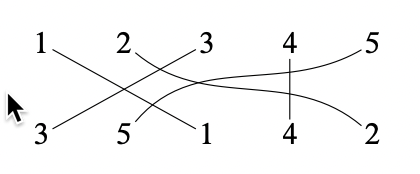
\includegraphics[width=.4\textwidth]{../images/GroupTheory/2.png}
\label{}
\end{figure}
is even
\end{remark}

For a permutation \(\sigma\), consider the products
\begin{align*}
V=\prod_{1\le i<j\le n}(j-i)=(2-1)(3-1)\dots(n-1)&\\
(3-2)\dots(n-2)&\\
\dots\quad&\\
(n-(n-1))&
\end{align*}
\begin{align*}
\sigma V=\prod_{1\le i<j\le n}(\sigma(j)-\sigma(i))=(\sigma(2)-\sigma(1))(\sigma(3)-\sigma(1))\dots(\sigma(n)-\sigma(1))&\\
(\sigma(3)-\sigma(2))\dots(\sigma(n)-\sigma(2))&\\
\dots\quad&\\
(\sigma(n)-\sigma(n-1))&
\end{align*}
Both products run over the 2-element subsets \(\{i,j\}\) of \(\{1,2,\dots,n\}\) and the terms
corresponding to a subset are the same except that each inversion introduces a negative sign.
Therefore
\begin{equation*}
\sigma V=\sgn(\sigma)V
\end{equation*}

Now let \(P\) be the additive group of maps \(\Z^n\to\Z\). For \(f\in P\) and \(\sigma\in S_n\), let \(\sigma f\)
denote the element of \(P\) defined by
\begin{equation*}
(\sigma f)(z_1,\dots,z_n)=f(z_{\sigma(1)},\dots,z_{\sigma(n)})
\end{equation*}
For \(z\in\Z^n\) and \(\sigma\in S_n\), let \(z^\sigma\) denote the element of \(\Z^n\) s.t. \((z^\sigma)_i=z_{\sigma(i)}\).
Then \((z^\sigma)^\tau=z^{\sigma\tau}\). By definition, \((\sigma f)(z)=f(z^\sigma)\), and
so \(((\sigma\tau)f)(z)=f(z^{\sigma\tau})=f((z^\sigma)^\tau)=(\tau f)(z^\sigma)=(\sigma(\tau f))(z)\), i.e.
\begin{equation*}
\sigma(\tau f)=(\sigma\tau)f
\end{equation*}

Let \(p\in P\) defined by
\begin{equation*}
p(z_1,\dots,z_n)=\prod_{1\le i<j\le n}(z_j-z_i)
\end{equation*}
The same argument as above shows that
\begin{equation*}
\sigma p=\sgn(\sigma)p
\end{equation*}
On putting \(f=p\), we finds that
\begin{equation*}
\sgn(\sigma)\sgn(\tau)=\sgn(\sigma\tau)
\end{equation*}
Therefore ``sign'' is a homomorhism \(S_n\to\{\pm 1\}\). When \(n\ge 2\), it is surjective, and so its
kernel is a normal subgroup of \(S_n\) of order \(\frac{n!}{2}\), called the \textbf{alternating
group} \(A_n\)

\begin{remark}
We show shown that there exists a homomorhism \(\sgn:S_n\to\{\pm 1\}\) s.t. \(\sgn(\sigma)=-1\) for every
transposition. The transposition generate \(S_n\), and so sign is uniquely determined by this
property. Now let \(G=\Sym(X)\), where \(X\) is a set with \(n\) elements. The choice of an
ordering of \(X\) determines an isomorphism of \(G\) with \(S_n\) sending transpositions to
transpositions. Therefore \(G\) also admits a unique isomorphism \(\epsilon:G\to\{\pm 1\}\) s.t. \(\epsilon(\sigma)=-1\)
for every transposition \(\sigma\). Once we have chosen an ordering of \(X\), we can speak of the
inversions of an element \(\sigma\) of \(G\), and define a sign homomorhism \(G\to\{\pm 1\}\) as before. This
must agree with \(\epsilon\), and so \(\epsilon(\sigma)\) equals 1 or \(-1\) according as \(\sigma\) has an even or an odd
number of inversions.
\end{remark}

A \textbf{cycle} is a permutation of the following form
\begin{equation*}
i_1\mapsto i_2\mapsto i_3\mapsto\dots\mapsto i_r\mapsto i_1
\end{equation*}
The \(i_j\) are required to be distinct. We denote this cycle by \((i_1 i_2\dots i_r)\) and call \(r\)
its \textbf{length}. The \textbf{support of the cycle} \((i_1\dots i_r)\) is the set \(\{i_1,\dots,i_r\}\) and cycles are
\textbf{disjoint} if their supports are disjoint. Disjoint cycles commute

\begin{proposition}[]
Every permutation can be written as a product of disjoint cycles
\end{proposition}

\begin{proof}
\(\sigma\in S_n\), and let \(O\subset\{1,\dots,n\}\) be an orbit for \(\la\sigma\ra\). If \(\abs{O}=r\), then for
any \(i\in O\),
\begin{equation*}
O=\{i,\sigma(i),\dots,\sigma^{r-1}(i)\}
\end{equation*}
Therefore \(\sigma\) and the cycle \((i\;\sigma(i)\dots\sigma^{r-1}(i))\) have the same action on any element of \(O\).
Let
\begin{equation*}
\{1,2,\dots,n\}=\bigcup_{j=1}^mO_j
\end{equation*}
be the decomposition of \(\{1,\dots,n\}\) into a disjoint union of orbits for \(\la\sigma\ra\), and let \(\gamma_j\)
be the cycle associated with \(O_j\). Then
\begin{equation*}
\sigma=\gamma_1\dots\gamma_m
\end{equation*}
is a decomposition of \(\sigma\) into a product of disjoint cycles.
\end{proof}

\begin{corollary}[]
Each permutation \(\sigma\) can be written as a product of transpositions; the number of transpositions
in such a product is even or odd according as \(\sigma\) is even or odd
\end{corollary}

\begin{proof}
\begin{equation*}
(i_1i_2\dots i_r)=(i_1i_2)\dots(i_{r-2}i_{r-1})(i_{r-1}i_r)
\end{equation*}
Because sign is a homomorhism, and the signature of a transposition is -1, \(\sgn(\sigma)=-1^{\#\text{transpositions}}\)
\end{proof}

\section{{\bfseries\sffamily TODO} skip and problems}
\label{sec:org1aac292}
\begin{center}
\begin{tabular}{lll}
\ref{SKIP} & \ref{SKIP2} & \ref{SKIP3}\\
\end{tabular}
\end{center}
\end{document}
